% !TEX root = thesis.tex
\documentclass[12pt,a4paper,titlepage,listof=totoc,bibliography=totoc,chapteratlists=0pt]{scrreprt}
\usepackage[utf8]{inputenc}
\usepackage[ngerman]{babel}
\usepackage{array}
\usepackage{ragged2e}
\usepackage{booktabs}

\newcolumntype{P}[1]{>{\RaggedRight\arraybackslash\hspace{0pt}}p{#1}}

\input{header}

\makeatletter
\def\bstctlcite{\@ifnextchar[{\@bstctlcite}{\@bstctlcite[@auxout]}}
\def\@bstctlcite[#1]#2{\@bsphack
	\@for\@citeb:=#2\do{%
		\edef\@citeb{\expandafter\@firstofone\@citeb}%
		\if@filesw\immediate\write\csname #1\endcsname{\string\citation{\@citeb}}\fi}%
	\@esphack}
\makeatother

\clubpenalty=10000 
\widowpenalty=10000
\displaywidowpenalty=10000
\interfootnotelinepenalty=10000

\title{Next-Level Relaunch der Schulhomepage: neuestes Design und aktuellste Animationen}
\author{Mona Angerer, Peter Klose}

\makeindex
\makeglossaries
\begin{document}
\bstctlcite{IEEEexample:BSTcontrol}
\newcommand{\reminder}[1]
{ \textcolor{red}{<[{\bf\marginpar{\mbox{$<==$}} #1 }]>} }
\newcommand{\icode}[1]{\lstinline$#1$}
%\urlstyle{same}
%\setstretch{1.5}
\setstretch {1.433}
\renewcommand{\arraystretch}{1.2}


\includepdf{./titlepage/coversheet}
\pagenumbering{Roman}
\newpage
\thispagestyle{empty}
\vspace{3cm}
~ \\ \\
Ich erkläre an Eides statt, dass ich die vorliegende Diplomarbeit selbstständig und ohne fremde Hilfe verfasst, andere als die angegebenen Quellen und Hilfsmittel nicht benutzt bzw. die wörtlich oder sinngemäß entnommenen Stellen als solche kenntlich gemacht habe.

Die Arbeit wurde bisher in gleicher oder ähnlicher Weise keiner anderen Prüfungsbehörde vorgelegt und auch noch nicht veröffentlicht.

Die vorliegende Diplomarbeit ist mit dem elektronisch übermittelten Textdokument identisch.
\vspace{3cm}
% Hier kommt die Unterschrift drüber
\begin{tabbing}
Leonding, April 2024 \hspace{5cm} M.Angerer \& P.Klose
\end{tabbing}
\vspace{10cm}
\newpage
\setcounter{page}{1}

\begin{spacing}{1}
    \chapter*{Abstract}
\end{spacing}
\begin{wrapfigure}{r}{0.3\textwidth}
    \begin{center}
      \includegraphics[width=0.2\textwidth]{pics/question_mark.png}
    \end{center}
\end{wrapfigure}
The present diploma thesis deals with the redesign of the school homepage of HTL Leonding, aiming to bring the design up to date and present the most important information logically and clearly.

The current version of the HTL Leonding homepage serves as the starting point for this work. An examination of the best designs available at the time of creation subsequently led to a rough draft of the website. This draft was then grouped into blocks that could be implemented in Storyblok. For each block, a corresponding representation was developed in Next.js.

This thesis illustrates the development of the website in the process as it was developed and provides insights into the technical background.
\newpage
\begin{spacing}{1}
    \chapter*{Zusammenfassung}
\end{spacing}
\begin{wrapfigure}{r}{0.3\textwidth}
    \begin{center}
      \includegraphics[width=0.2\textwidth]{pics/question_mark.png}
    \end{center}
\end{wrapfigure}
Die vorliegende Diplomarbeit beschäftigt sich mit der Neugestaltung der Schulhomepage der HTL Leonding, mit dem Ziel, das Design auf den neuesten Stand zu bringen und die wichtigsten Informationen logisch und übersichtlich darzustellen.

Die aktuelle Version der HTL Leonding Homepage bildet den Ausgangspunkt dieser Arbeit. Eine Auseinandersetzung mit den besten Designs zum Zeitpunkt der Erstellung führte anschließend zu einem Grobentwurf der Webseite. Dieser Entwurf wurde dann in Blöcke gruppiert, die anschließend in Storyblok implementiert werden konnten. Für alle Blöcke wurde dann eine entsprechende Darstellung in Next.js entwickelt.

Diese Arbeit zeigt die Entstehung der Webseite in dem Ablauf, wie sie entwickelt wurde, und bietet Einblicke in den technischen Hintergrund.


\pagestyle{plain}

\renewcommand{\lstlistlistingname}{Quellcodeverzeichnis}

\tableofcontents
\newpage
\setcounter{RPages}{\value{page}}
\setcounter{page}{0}
\pagenumbering{arabic}
\pagestyle{scrheadings}

\begin{spacing}{1}
\chapter{Einleitung}\label{chapter:introduction}
\end{spacing}
\section{Abkürzungen}

Um zu Kennzeichnen, welche Abschnitte der Diplomarbeit von wem verfasst wurden,
werden in den Überschriften der Kapitel die Buchstaben M für Mona Angerer und P für Peter Klose
hinzugefügt. Wenn kein Autor angeführt wird, ist der folgende Abschnitt von 
Beiden geschrieben.


\section{Ausgangssituation}

Seit dem Jahr 20xx verfügt die HTL Leonding über eine Website, 
die damals ebenfalls von SchülerInnen entwickelt wurde und auf Wordpress basiert. 

\begin{figure}
    \centering
    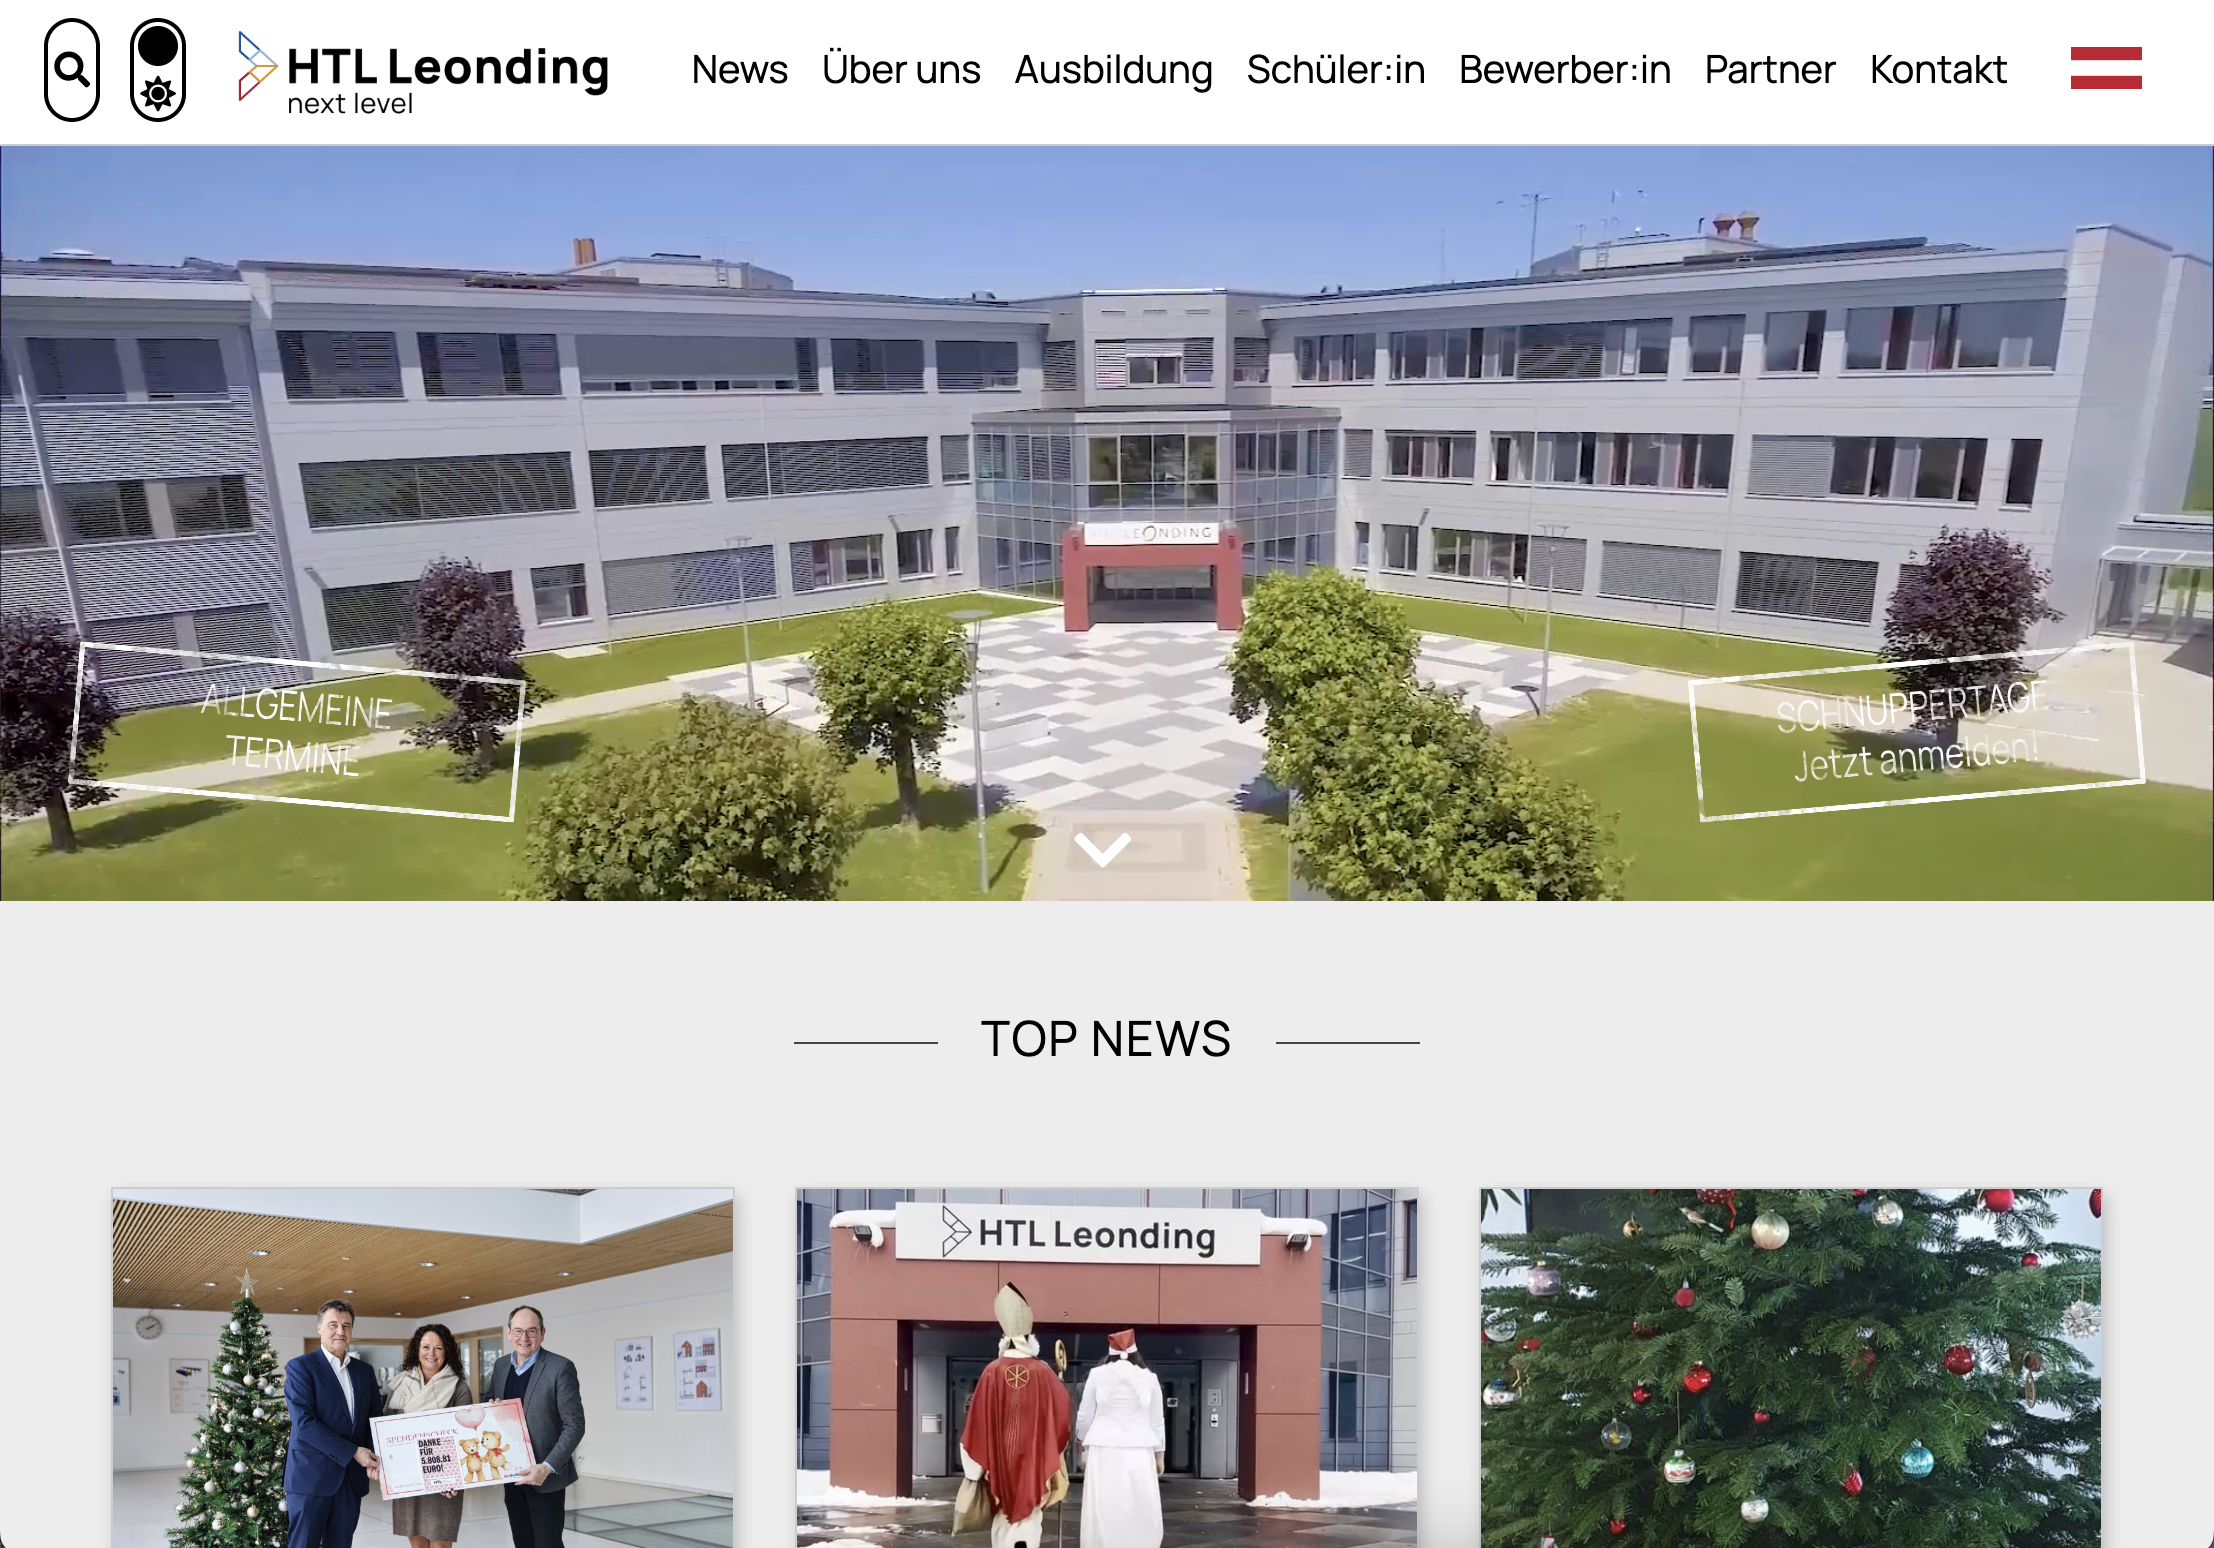
\includegraphics[scale=0.3]{pics/startseite_ausgangslage.png}
    \caption{Startseite Ausgangssituation}
    \label{fig:impl:startseite_ausgangslage}
\end{figure}


\section{Problemstellung}

Die HTL Leonding-Website, die 20xx von Schülern auf Wordpress-Basis entwickelt wurde, 
zeigt eine durchaus den Anforderungen einer Schulhomepage entsprechenden, 
jedoch in die Jahre gekommene Plattform. Die technischen Möglichkeiten und Designstandards haben 
sich in den letzten Jahren erheblich weiterentwickelt, was dazu führt, dass die aktuelle 
Website nicht mehr den zeitgemäßen Ansprüchen entspricht. 

Die bestehende Website weist Unstimmigkeiten in der Benutzerführung auf, 
insbesondere im Hinblick auf die Menüstruktur, die als unübersichtlich wahrgenommen wird. 
Usern fällt es schwer, sich auf der Oberfläche zurechtzufinden und den gesuchten Inhalt auf Anhieb zu finden. 
Während mancher Content nur schwer zu finden ist, weist die Homepage auch über Inhalte auf, 
die an mehreren Stellen und unterschiedlichen Unterseiten zu finden ist. Dies verstärkt zusätzlich 
die Verwirrung und schlechte intuitive Handhabung. Zudem verfügt sie über lange Ladezeiten, was die 
Benutzererfahrung deutlich beeinträchtigt. Durch die langen Unterbrechungen, 
die in der Bedienung entstehen könnten und die immer kürzer werdende Aufmerksamkeitsspanne und Ungeduld der Menschen, 
könnte es nicht nur zu einer getrübten Stimmung, sondern sogar zum Verlassen der Website kommen. Das Design erscheint 
zu bunt und durch die vielen Bilder Videos, die oftmals einen Großteil der Seite einnehmen, 
wirkt der Webauftritt der HTL Leonding überladen und nicht mehr zeitgemäß. Des Weiteren folgt die Webanwendung einem strikten
Box-Design, was fehlende Dynamik zur Folge hat und eintönig wirkt. Auch im Mobile-Modus gibt es zudem Herausforderungen,
wie schwierige Bedienung des Menüs und Schwierigkeiten beim Zurechtfinden und Navigieren. Da immer mehr Menschen eher auf 
ihren Mobilgeräten und nicht nur ihren PCs und Laptops Webseiten aufrufen, gewinnt insbesondere dies progressiv an Bedeutung.

Es hat sich gezeigt, dass die Website möglicherweise nicht mehr effektiv die Bedürfnisse und 
Ziele der verschiedenen Nutzergruppen erfüllt. Die Schulleitung hat angesichts dieser Erkenntnisse den Vorschlag gemacht, 
im Rahmen einer Diplomarbeit einen neuen Webauftritt zu gestalten. Dies bietet die Chance, die bestehenden 
Herausforderungen zu adressieren, die Website zu modernisieren und eine verbesserte Benutzererfahrung für alle Zielgruppen zu schaffen.


\section{Aufgabenstellung und Ziele}

Um ein breites Spektrum an Technologien abzudecken und unterschiedliche Ansätze zu fördern, werden zwei Teams mit dieser Diplomarbeit betraut. 
Diese Herangehensweise ermöglicht es, verschiedene Ideen und Lösungsansätze zu erforschen und so eine fundierte Grundlage für die Gestaltung 
des neuen Webauftritts der HTL Leonding zu schaffen.

Die Vorgabe besteht darin, als Backend das headless CMS Storyblok zu verwenden. Die Motivation hinter dieser Entscheidung 
liegt in der aktuellen Relevanz und Flexibilität dieses Content Management Systems. Die SchülerInnen werden dazu ermutigt, 
sich eingehend über verschiedene Frontend-Varianten zu informieren und dazu zu recherchieren, um diejenige zu finden, 
die sich am besten mit Storyblok kombinieren lässt und den Anforderungen am besten gerecht wird.
Die neue Website soll eine mit entsprechende Backend-Struktur aufgebaut sein, so dass
sie für die Zukunft eine leichte Wartung ermöglicht. 
Um die Benutzerfreundlichkeit zu erhöhen wird gefordert, den Content besser zu strukturieren,
abzuwägen, welche Inhalte ins LeoWiki ausgelagert werden sollen und die Inhalte so zu 
platzieren, dass eine intuivtive Navigation für alle Benutzergruppen ermöglicht wird.
Das Design der Website soll an die derzeitigen Standards und Trends angepasst werden
und mithilfe von Animationen und spannendem Design einladend und ansprechend gestaltet werden.

Das endgültige Ziel ist eine technisch sauber gelöste, gut strukturierte, ansprechend gestaltete
Weboberfläche, die eine einfache und intuitive Navigation ermöglicht. Alle relevanten Inhalte, die die HTL Leonding repräsentieren,
sind auf der Homepage zu finden und bilden ein einladendes Bild der HTL Leonding. 

\begin{spacing}{1}
\chapter{Design}
\end{spacing}
Eines der Hauptthemen der Diplomarbeit ist die Überarbeitung des bisherigen Designs. 
Um dies zu erreichen, werden nicht nur über die aktuellen Standards und Trends analysiert, 
der aktuelle Content der Website restrukturiert und Usability-Tests durchgeführt, 
sondern auch ein mehrstündiger Workshop zum Thema UI/UX Design an der JKU absolviert.

\section{Recherche} \label{sec:Recherche}
\setauthor{Angerer Mona}
Um ein umfassendes Verständnis für die derzeit gängigen Designmethoden erhalten zu können, wurden zahlreiche bekannte große Websites wie die von Apple (....) und anderen analysiert.
Dabei werden die überschneidenden Merkmale identifiziert und herausgearbeitet und diejenigen, die für die HTL-Website besonders relevant sind, anschließend genauer untersucht. 
Auffällig ist dabei die übergeordnete Präferenz für das Motto „Weniger ist mehr“. Durchgehend dominiert minimalistisches Design mit vielen weißen Flächen, wodurch ein edler, strukturierter Eindruck erweckt wird.

Im Kontrast dazu werden jedoch auch viele Vektor- oder svg-Animationen, oftmals auch im „handgezeichneten“ Stil, verwendet, die das saubere Layout auflockern und Bewegung in die Benutzeroberfläche bringen. 

Darüber hinaus gewinnen Scrollingeffekte zunehmend an Bedeutung und werden von immer mehr Unternehmen als wichtiges und vielseitig einsetzbares Designelement betrachtet. 
Ob Parallax-Effekte, Scrollitelling, Immersive oder Horizontal Scrolling – das Weiterscrollen wird nicht mehr nur als „Bildschirminhalt verschieben“ gesehen, 
sondern wird zu einem immer wichtigeren, vielseitig eingesetzten Element. 

Ein weiterer interessanter Trend ist die verstärke Aufmerksamkeit auf individuell gestaltete
Error-Seiten. Diese werden zunehmend in das Gesamtdesign der Website integriert und mit kleinen 
Spielereien wie Animationen oder Mini-Games ausgeschmückt. 

Geometrische Ästhetik, insbesondere abstrakte Formen wie Dreiecke, 
Kreise, Vierecke oder eine Kombination davon, gewinnen im Web-Bereich deutlich sichtbar an Popularität. 
Auf vielen hochwertigen Websites tragen diese geometrischen Gestaltungselemente dazu bei, eine strukturierte und interessante Oberfläche zu schaffen. 


\section{Content-Strukturierung}
\setauthor{Angerer Mona}
Durch Gespräche mit SchülerInnen, Lehrkräften und InteressentInnen stellt sich hinaus, dass einer der am häufigsten bemängelten Aspekte der bisherigen 
HTL-Website der unübersichtliche Aufbau mit etlichen Unterseiten ist. Es fällt den Usern teilweise schwer, sich auf der Benutzeroberfläche zu orientieren 
und den gesuchten Inhalt auf Anhieb zu finden. Um dieses Problem zu beheben, wird zunächst eine eingehende Analyse des Menüs und seiner Unterpunkte durchgeführt, 
um einen umfassenden Überblick über den gesamten Website-Inhalt zu erhalten. Nach intensiver Prüfung wird anschließend festgestellt, dass durch eine Neustrukturierung von 
7 Menüpunkten auf nur noch 5 Hauptseiten übergegangen werden kann.

Des Weiteren wird ein erheblicher Teil des Inhalts von der Website ins LeoWiki, das interne Wiki der HTL Leonding, ausgelagert. 
Dies verhindert, dass Content, der nur für Personen, die bereits an der HTL Leonding lernen oder lehren, relevant ist, für Außenstehende sichtbar ist und ermöglicht, 
dass die meisten Seiten keine weiteren Unterseiten besitzen und somit als One Pager fungieren, auf denen der Inhalt durch einfaches Scrollen zugänglich ist.



\section{Workshop}
\setauthor{Angerer Mona}
An dem Workshop auf dem Campus der JKU, der von … von der Firma KBC abgehalten wurde, nahmen beiden Diplomarbeitsteams, der Betreuungslehrer Herr Professor Huemer und die beiden Professorinnen 
Frau Engleitner und Frau Rammelmüller teil. 

Um einen Ausgangspunkt für die Entwicklung eines Designkonzepts zu schaffen, 
führt man zunächst eine umfassende Problemanalyse durch (Siehe Abbildung \ref{fig:impl:problemanalyse}). In Teams wird die bewährte Post-It-Methode angewendet, 
bei der jeder/jede TeilnehmerIn unterschiedlich farbige Zettel erhält, um Mängel und Verbesserungsvorschläge auf gemeinsame Plakate zu kleben. 
Dieser kollaborative Ansatz ermöglicht die Erstellung einer Art Mindmap, auf der die Schwächen der aktuellen HTL-Website deutlich herausgearbeitet werden. 
Dabei werden Herausforderungen wie die Unübersichtlichkeit des Menüs, eine zu bunte Gestaltung und Probleme im Mobile-Modus hervorgehoben. 
Diese Methode lenkt den Fokus von Anfang an auf die Lösungsfindung in Beachtung der bereits existierenden Probleme, um somit nicht nur eine Neuimplementierung, 
sondern eine konkrete Verbesserung der Website zu erreichen.

\begin{figure}
    \begin{minipage}[b]{.4\linewidth} 
       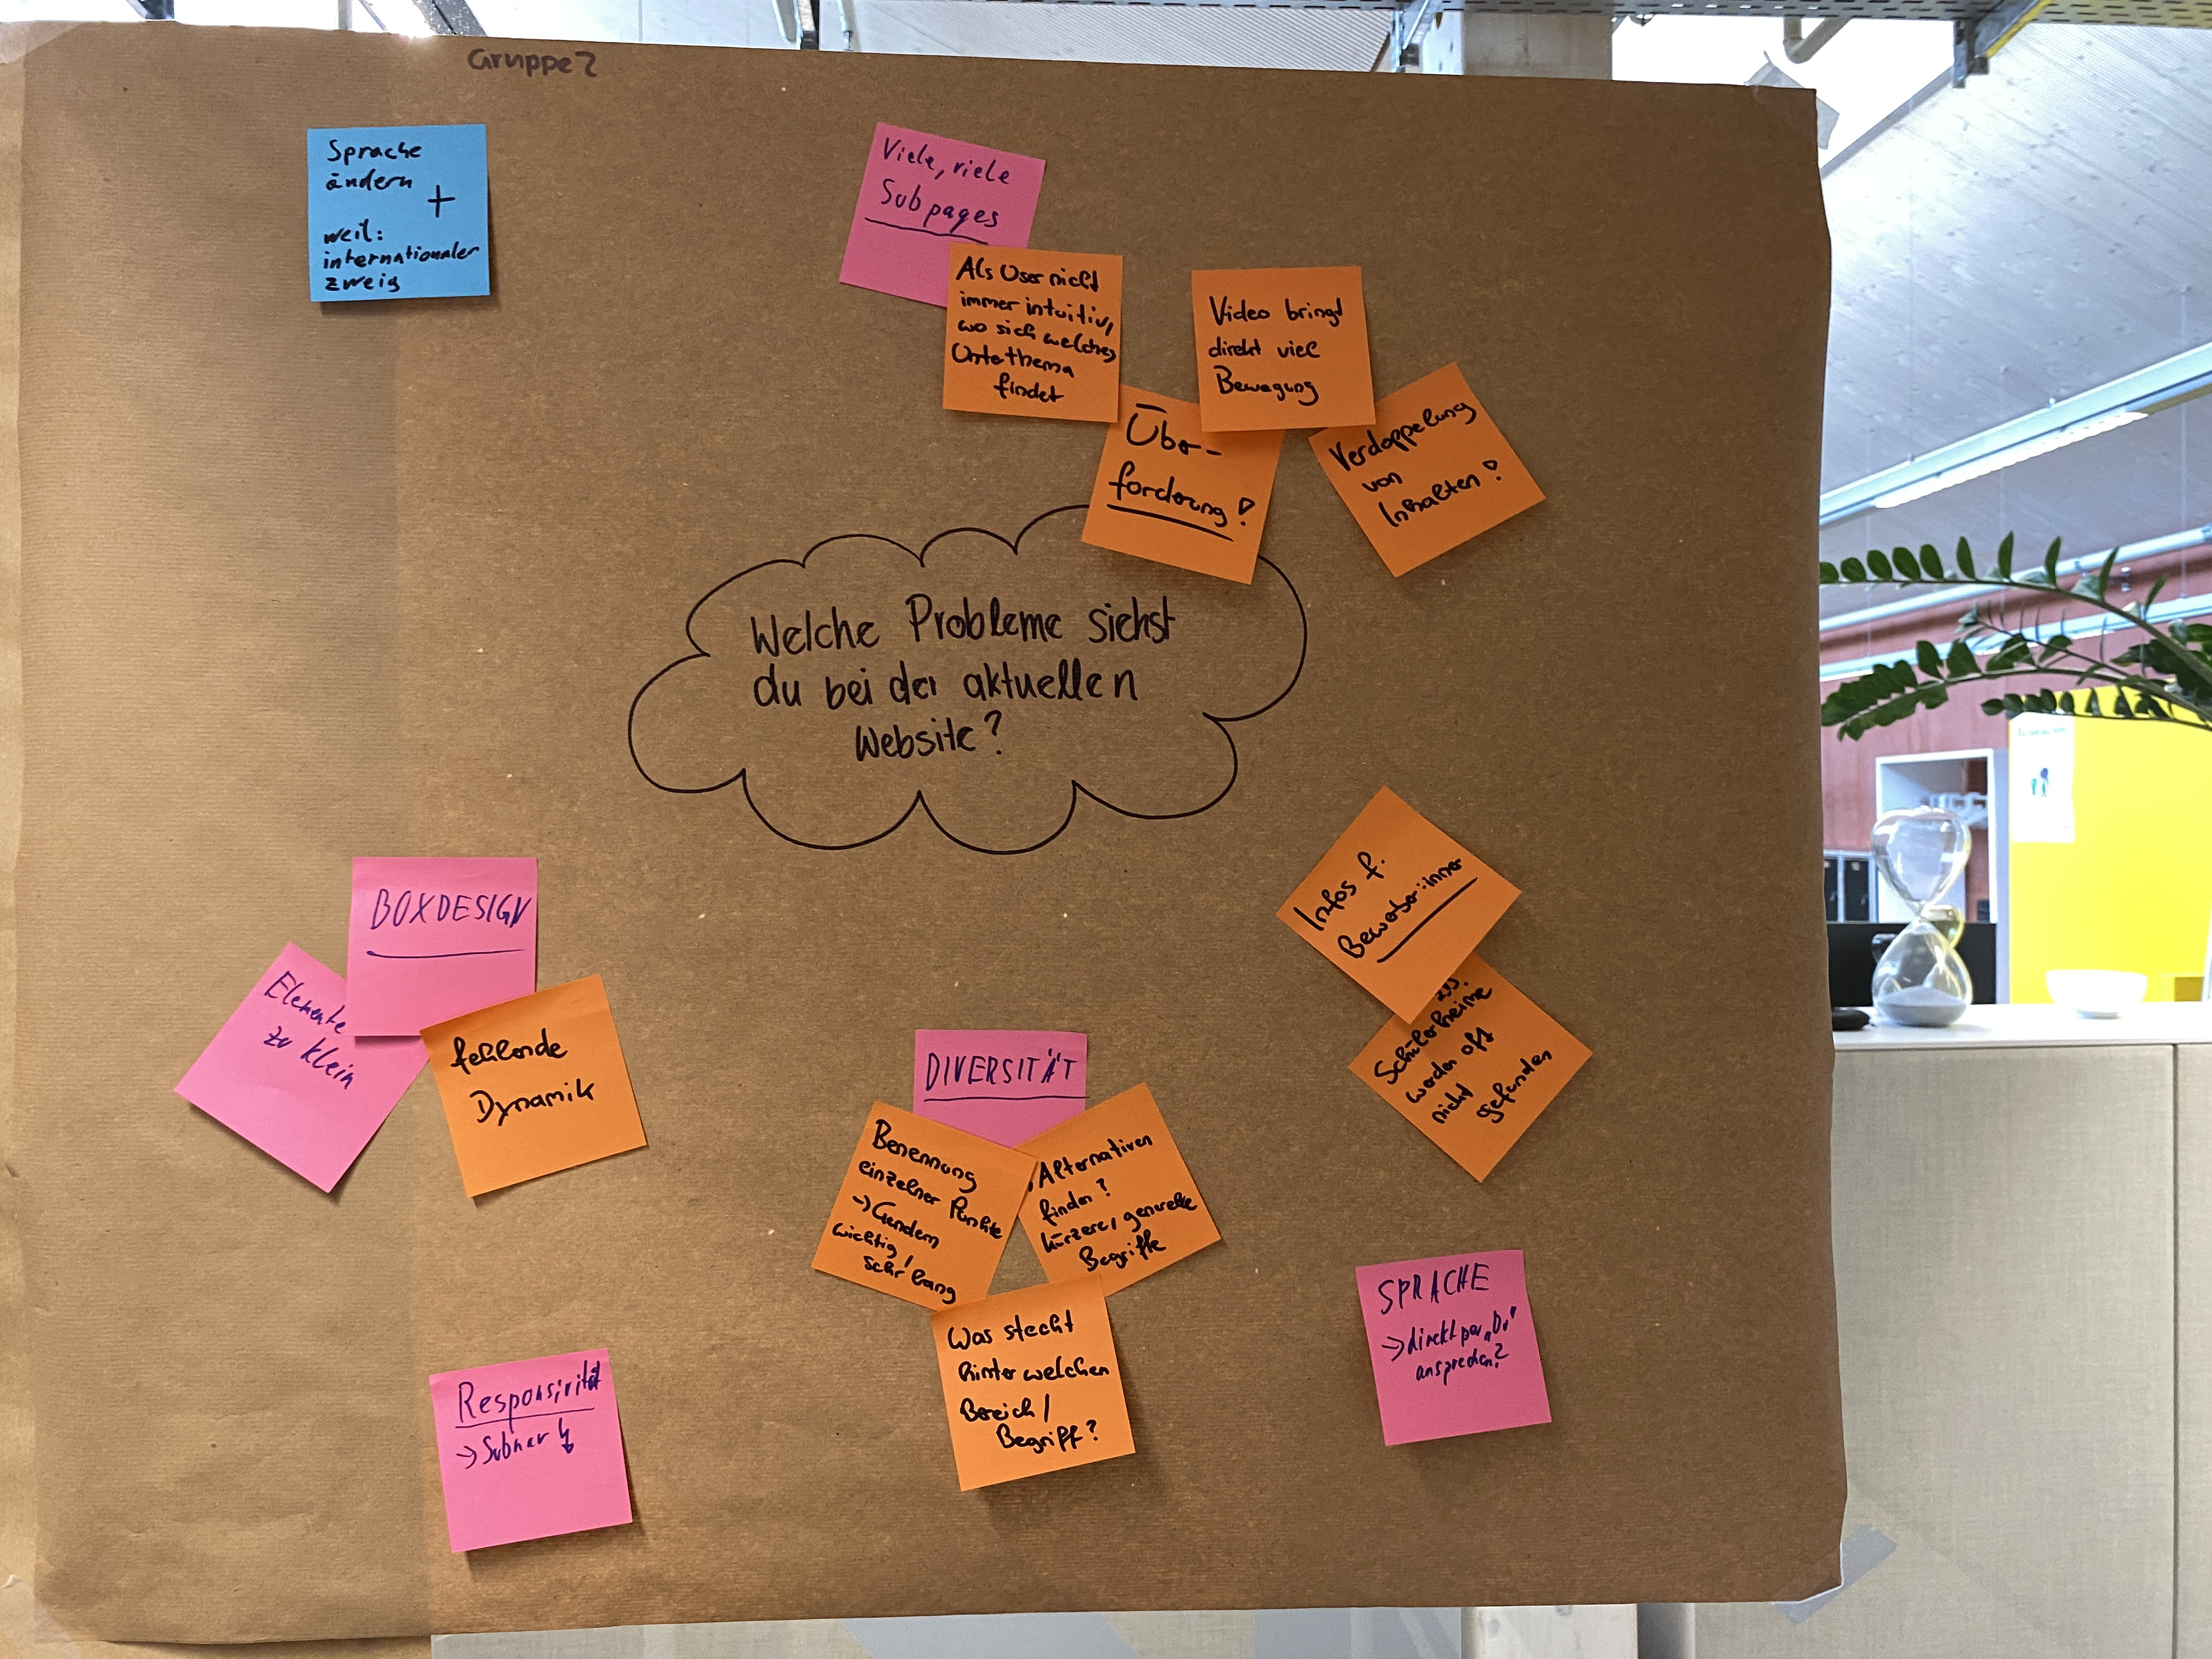
\includegraphics[width=\linewidth]{pics/problemanalyse.jpg}
       \caption{Problemanalyse}
       \label{fig:impl:problemanalyse}
    \end{minipage}
    \hspace{.05\linewidth}
    \begin{minipage}[b]{.4\linewidth}
       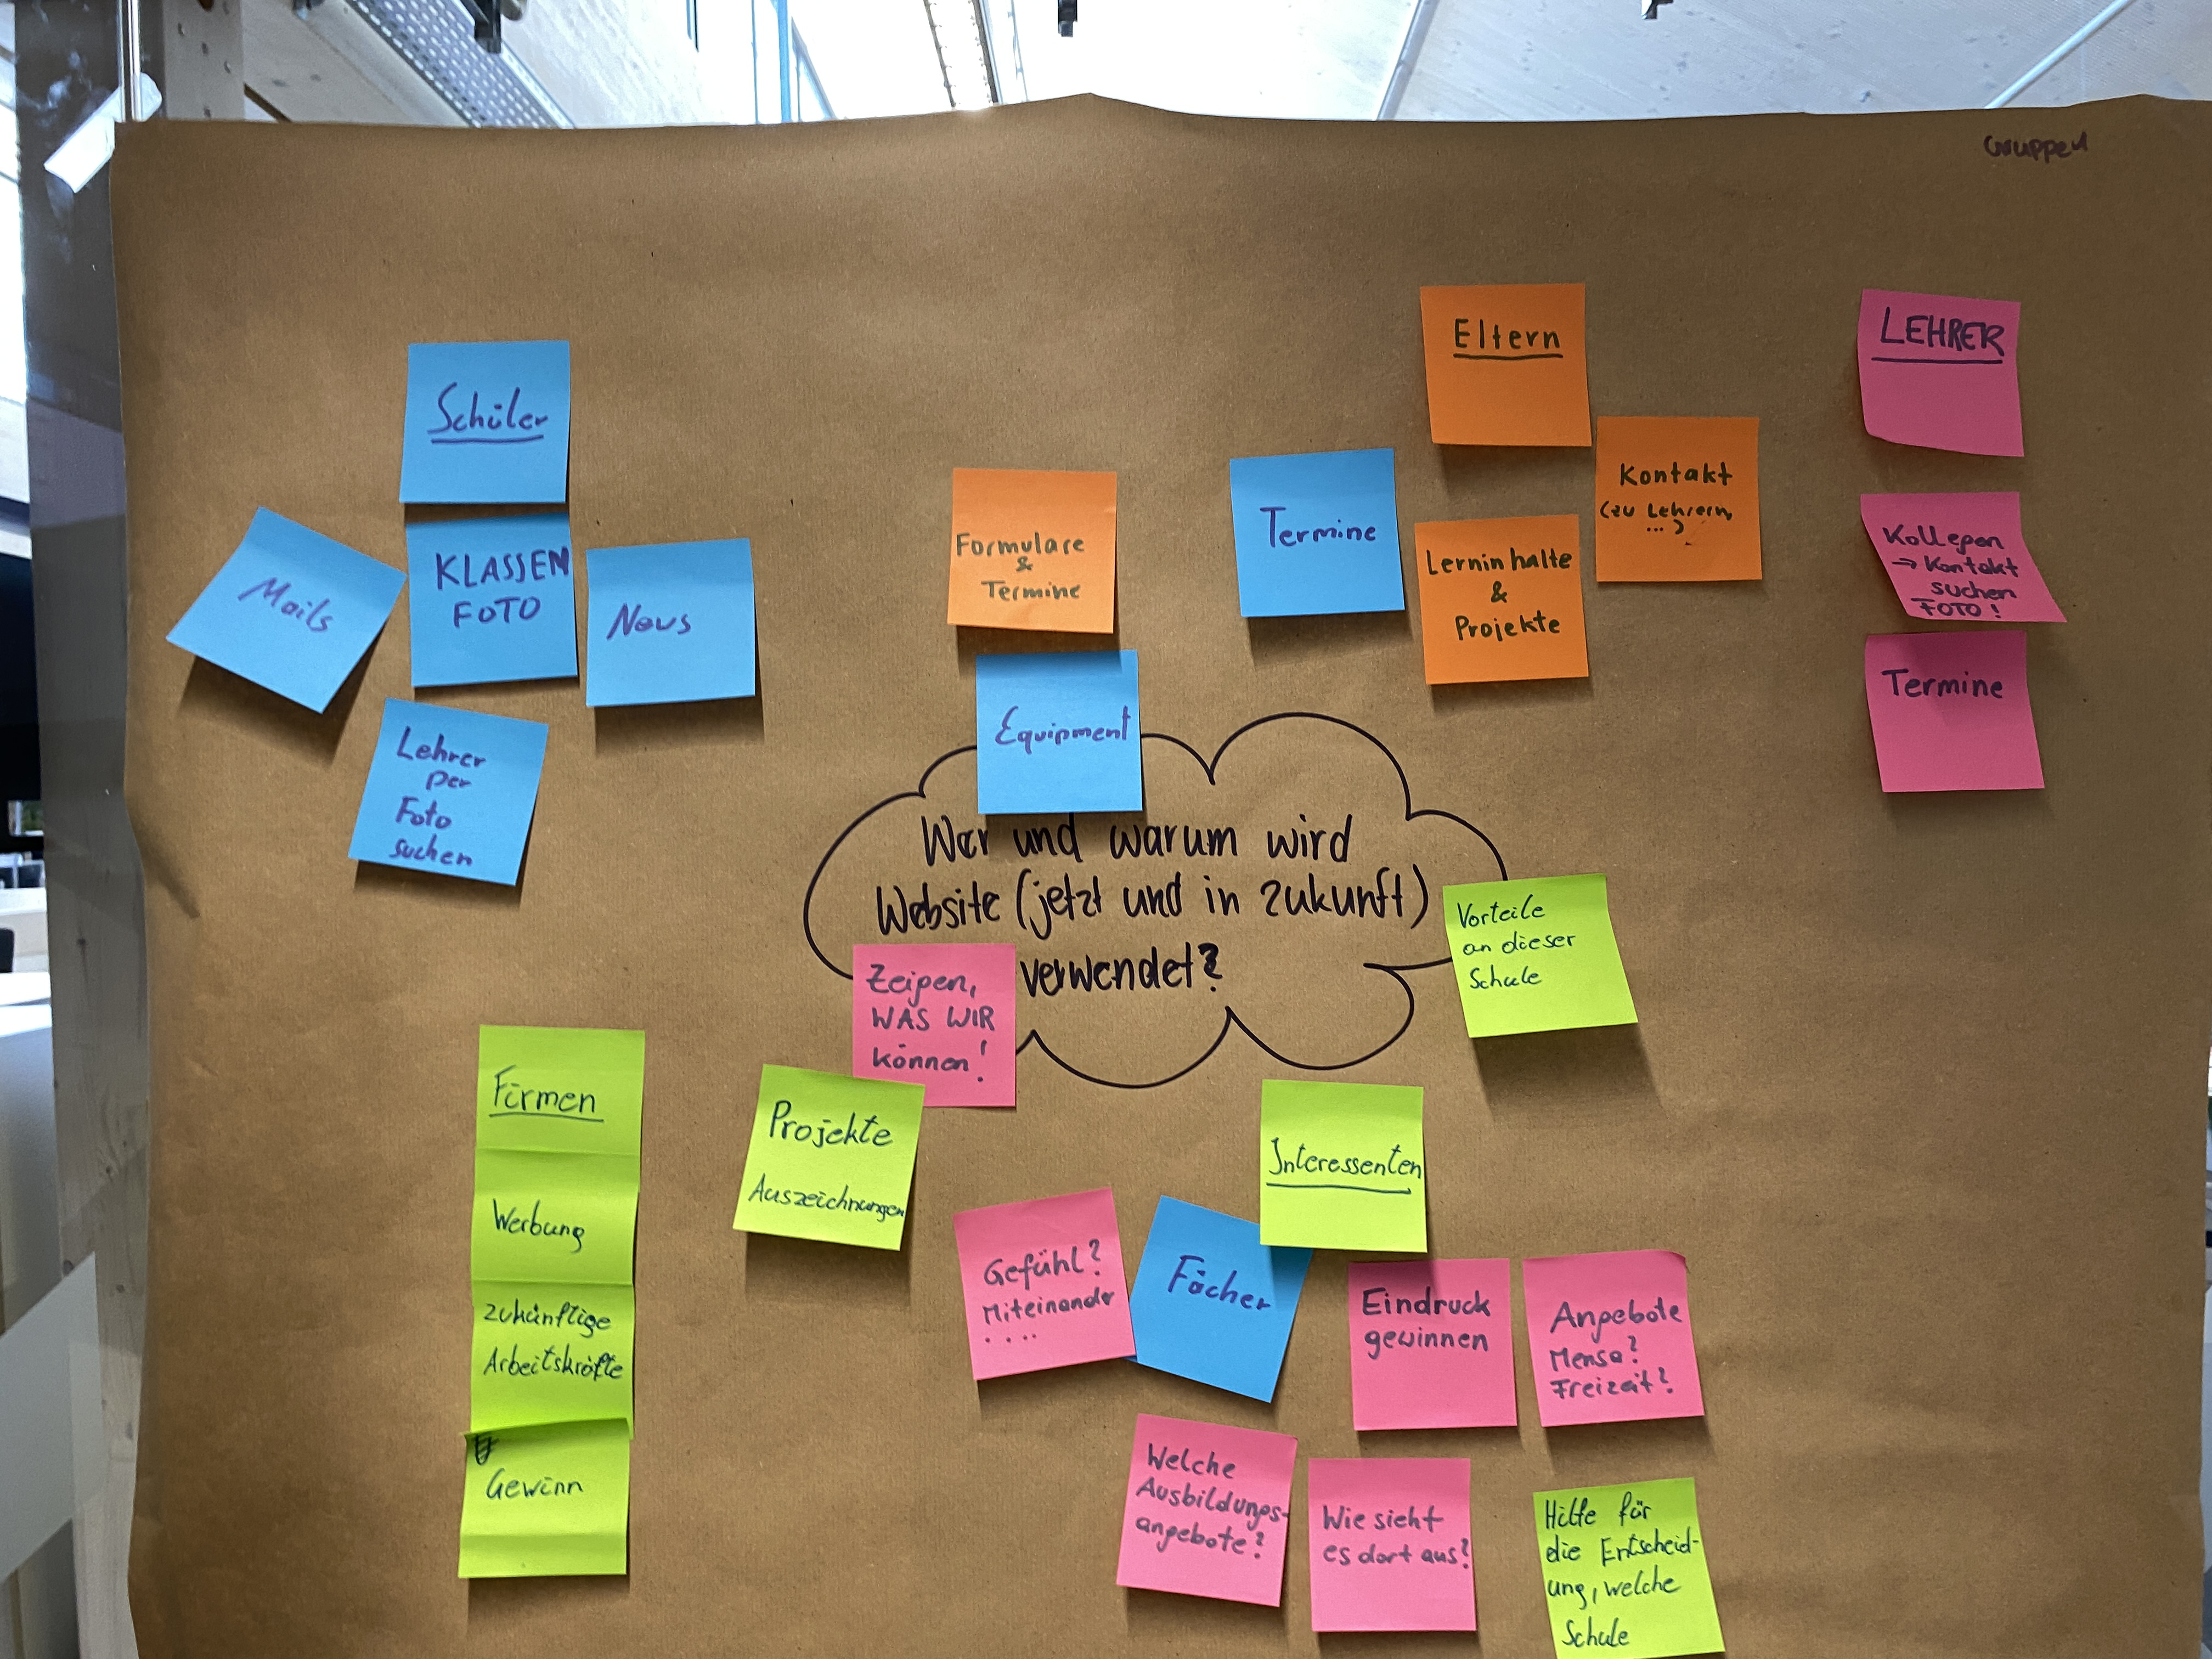
\includegraphics[width=\linewidth]{pics/zielgruppenanalyse.jpg}
       \caption{Zielgruppenanalyse}
       \label{fig:impl:zielgruppenanalyse}
    \end{minipage}
 \end{figure}

Der kreative kollaborative Prozess setzt sich fort und mündet in einer detaillierten Zielgruppenanalyse (Siehe Abbildung \ref{fig:impl:zielgruppenanalyse}). 
Dieser Schritt ist von besonderer Bedeutung in der Designentwicklung, da eine Benutzeroberfläche erst dann als gelungen betrachtet werden kann, 
wenn sie von den BenutzerInnen intuitiv genutzt werden kann und ihren individuellen Anforderungen gerecht wird. 
Bei der HTL-Website werden verschiedene Benutzergruppen identifiziert, darunter SchülerInnen, LehrerInnen, InteressentInnen, Firmen und Eltern. 
Zusätzlich berücksichtigt man deren spezifische Intentionen. Beispielsweise ist für Unternehmen von großem Interesse, 
welche Projekte an der Schule verfolgt werden und welche Technologien dafür verwendet werden. 
Eltern und InteressentInnen wiederum möchten vorrangig Informationen zu den angebotenen Zweigen und Fächern an der HTL erhalten, 
während Lehrkräfte und SchülerInnen insbesondere anstehende Events und Aktivitäten im Blick haben möchten. 
Diese präzise Zielgruppenanalyse bildet die Grundlage für ein benutzerzentriertes Designkonzept, das den Bedürfnissen aller Zielgruppen gerecht wird.


Um die Benutzerperspektive noch intensiver zu erfassen, geht man im weiteren Verlauf darauf ein, 
welche Gedanken, Wünsche, Handlungen und Emotionen die NutzerInnen während der Verwendung der Website durchlaufen (Siehe Abbildung \ref{fig:impl:user_gefühle}). 
Dabei werden nicht nur positive Gefühle und Gedanken, wie Vorfreude und Neugierde, herausgearbeitet, sondern auch potenzielle Ängste oder Unsicherheiten. 
Hierzu gehören beispielsweise Fragen wie: \glqq Bin ich gut genug für die HTL?\grqq oder \grqq Habe ich überhaupt Chancen, aufgenommen zu werden?\grqq.

Die Berücksichtigung dieser vielschichtigen Nutzererfahrungen ermöglicht eine empathische Gestaltung der Benutzeroberfläche, 
die nicht nur informativ ist, sondern auch dazu beiträgt, positive Emotionen zu fördern und mögliche Ängste zu mildern. 
Durch diese eingehende Analyse der Nutzerperspektive wird die HTL-Website nicht nur funktional, sondern auch emotional ansprechend und unterstützend gestaltet.

\begin{figure}
   \begin{minipage}[b]{.4\linewidth} 
      \includegraphics[width=\linewidth]{pics/user_gefühle_gedanken.JPG}
      \caption{UserInnen Gefühle}
      \label{fig:impl:user_gefühle}
   \end{minipage}
   \hspace{.05\linewidth}
   \begin{minipage}[b]{.4\linewidth}
      \includegraphics[width=\linewidth]{pics/user_missionen.JPG}
      \caption{UserInnen Missionen}
      \label{fig:impl:user:missionen}
   \end{minipage}
\end{figure}

Um eine intuitive Benutzererfahrung auf der Website sicherzustellen, werden darüber hinaus potenzielle Missionen, 
Gedankengänge und Vorgehensweisen der NutzerInnen berücksichtigt, die sie bei ihrem Besuch auf dem HTL-Webauftritt haben könnten (Siehe Abbildung \ref{fig:impl:user:missionen}). 
Es wurde dabei analysiert, welche konkreten Ziele sie verfolgen, welche Informationen sie suchen und welche Schritte sie wahrscheinlich unternehmen möchten.

Diese detaillierte Betrachtung der Nutzerinteraktion ermöglicht es, die Benutzeroberfläche so zu gestalten, dass sie den natürlichen Denk- und Handlungsmustern 
der BenutzerInnen entspricht. Durch das Verstehen der potenziellen Missionen und Gedankengänge wird sichergestellt, dass die Website nicht nur informativ ist, 
sondern auch nahtlos in den individuellen Ablauf der NutzerInnen integriert wird. Dieser Ansatz fördert eine reibungslose und effektive Nutzung der Website.

Mit dem erlangten Wissen über die zu behebenden Probleme und die unterschiedlichen Usergruppen, deren individuelle Anforderungen 
an die HTL-Website, die Ziele, die sie mit dem Besuch der Website verfolgen möchten und die Emotionen und Eindrücke, die man in den Usern beim benutzen der Oberfläche erwecken will,
wird nun der Startpunkt für die Erstellung eines Designentwurfs erleichtert. Dazu wurde unter den
TeilnehmerInnen des Workshops Zettel und Stifte ausgeteilt, um Skizzen und mögliche Layouts für die Weboberfläche zu gestalten. (Siehe Abbildung \ref{fig:impl:erste_entwuerfe})
Durch diese Methode werden eine Vielzahl an Ideen erbracht, die in der gesamten Gruppe geteilt und diskutiert werden. 
Dieser kreative Ansatz ermöglicht es, die gewonnenen Erkenntnisse 
unmittelbar in konkrete visuelle Konzepte umzusetzen und so den Grundstein für eine optimierte HTL-Website zu legen.

\begin{figure}
   \centering
   \begin{subfigure}{0.3\textwidth}
     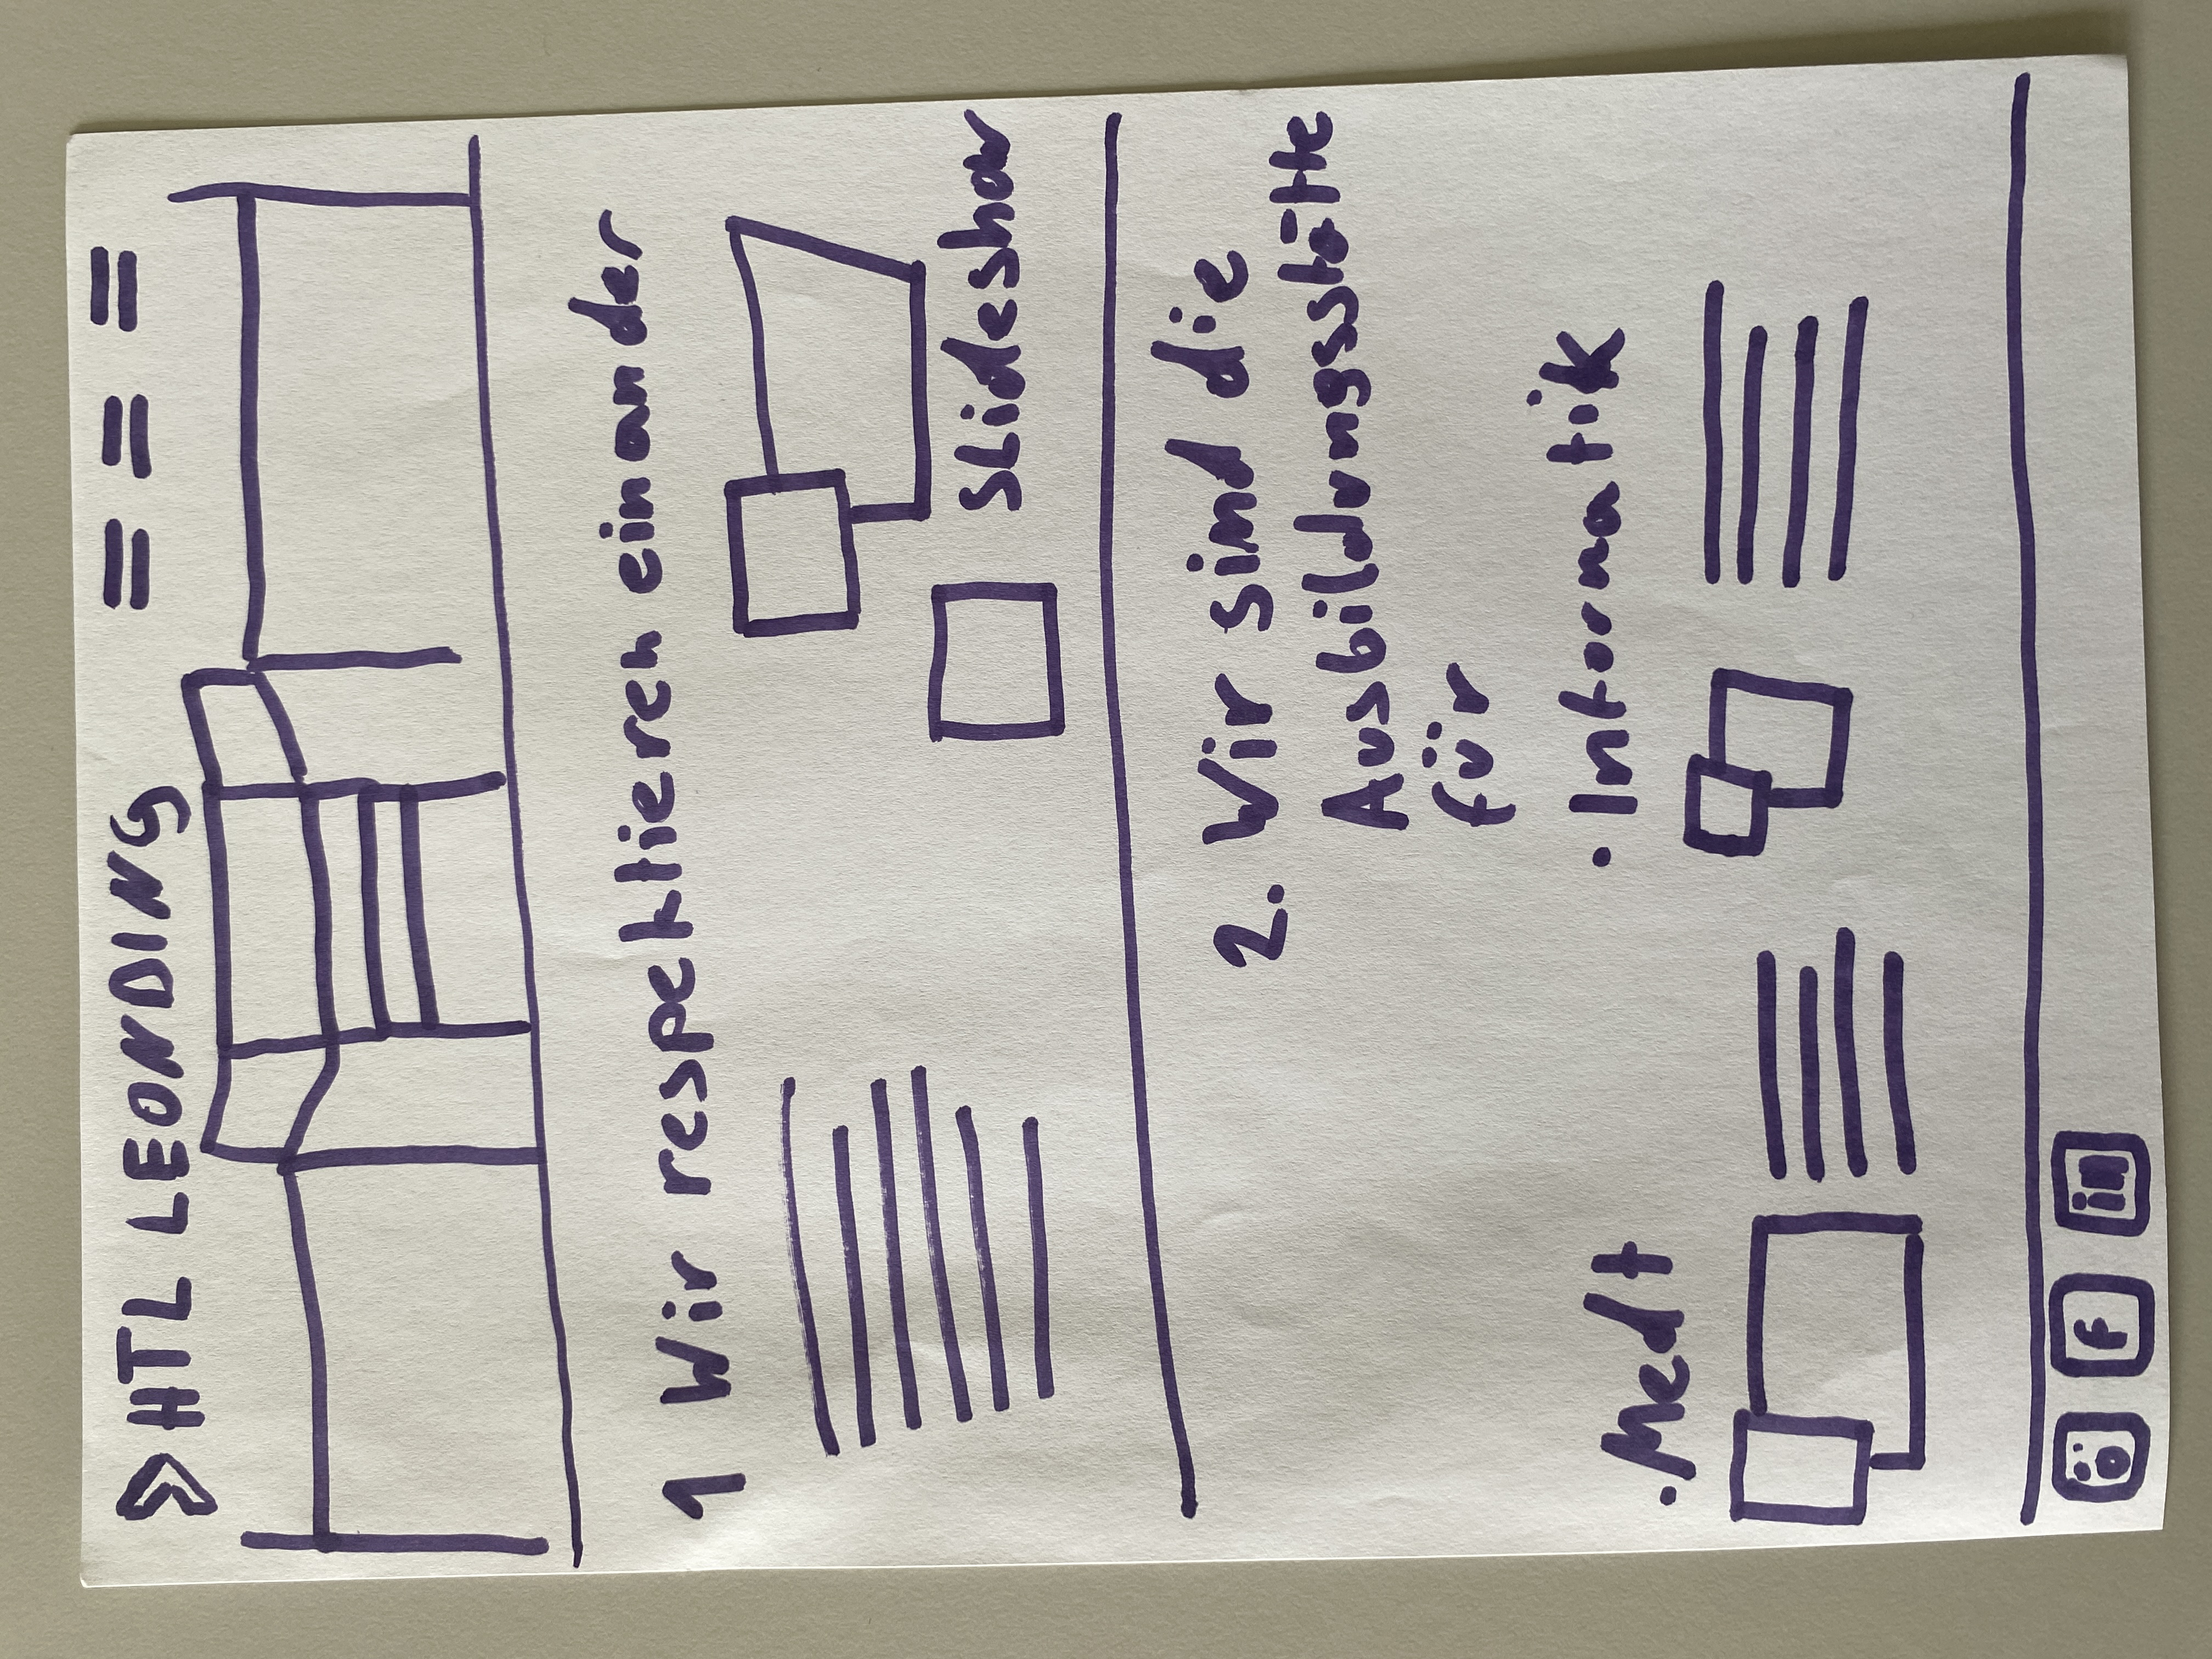
\includegraphics[width=\textwidth, angle=270]{pics/Entwurf_Beispiel_1.JPG}
     \caption{Entwurf 1}
     \label{fig:a}
   \end{subfigure}
   \hfill
   \begin{subfigure}{0.3\textwidth}
     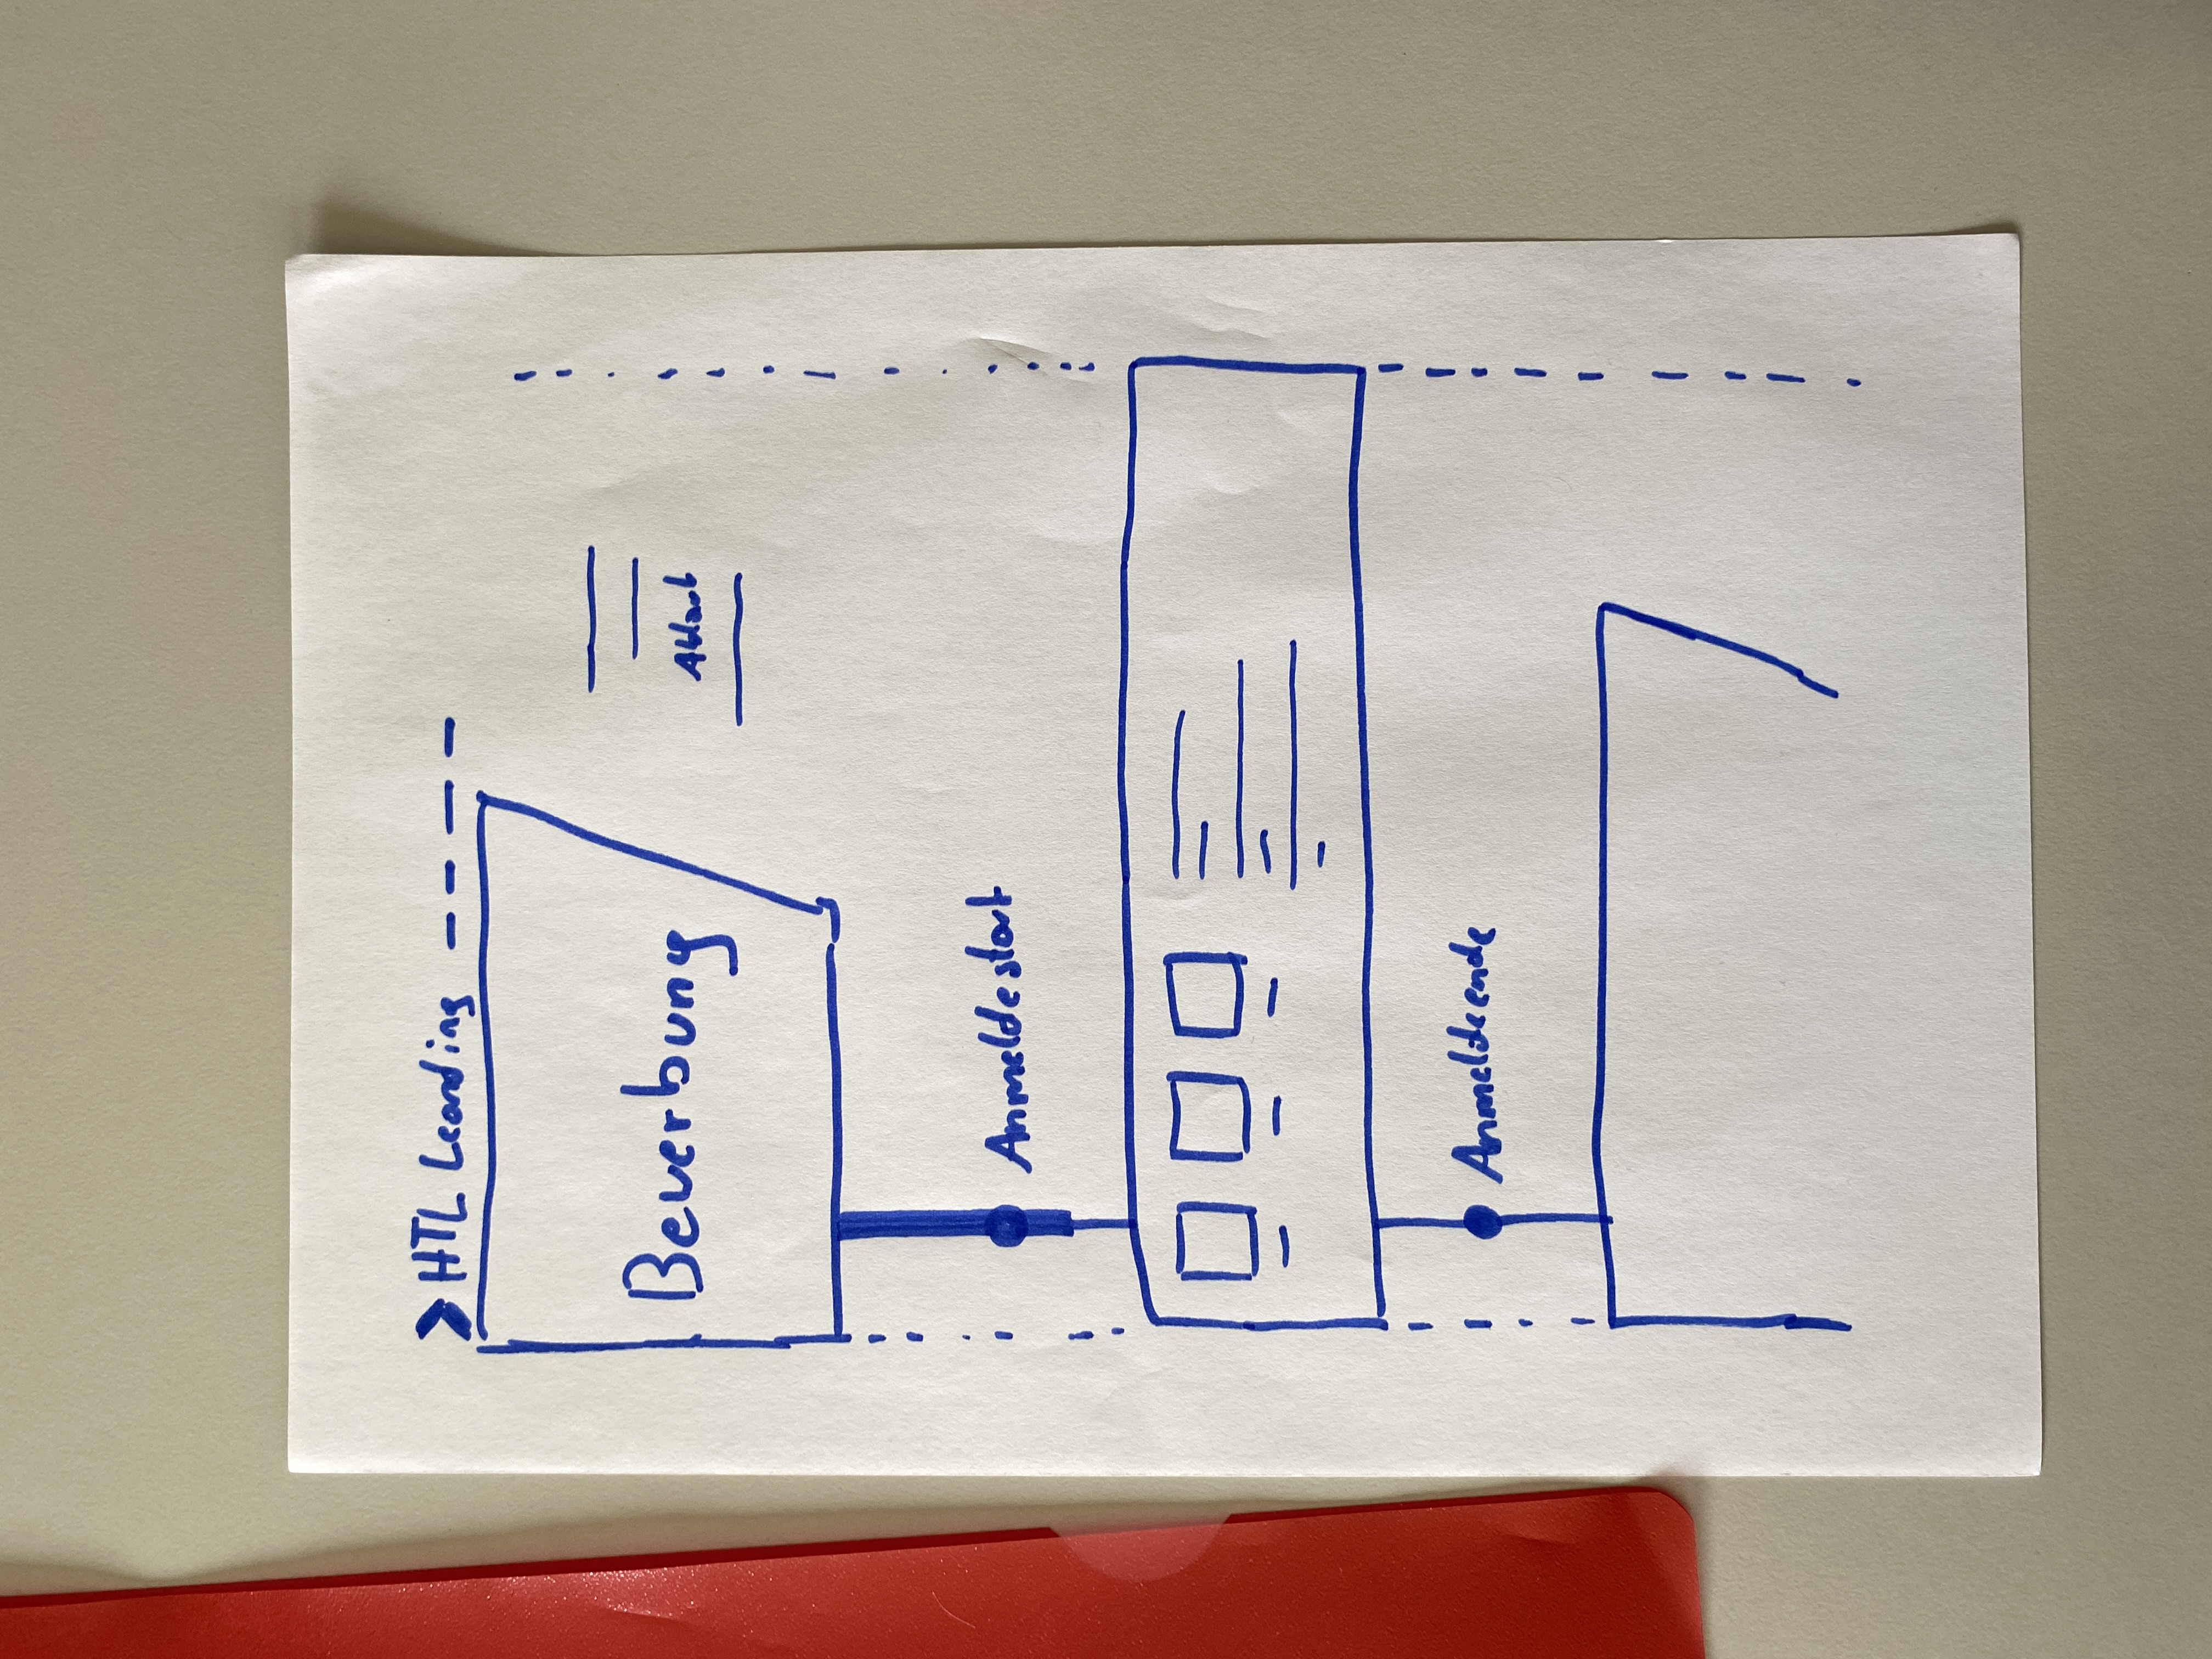
\includegraphics[width=\textwidth, angle=270]{pics/Entwurf_Beispiel_2.JPG}
     \caption{Entwurf 2}
     \label{fig:b}
   \end{subfigure}
   \hfill
   \begin{subfigure}{0.3\textwidth}
     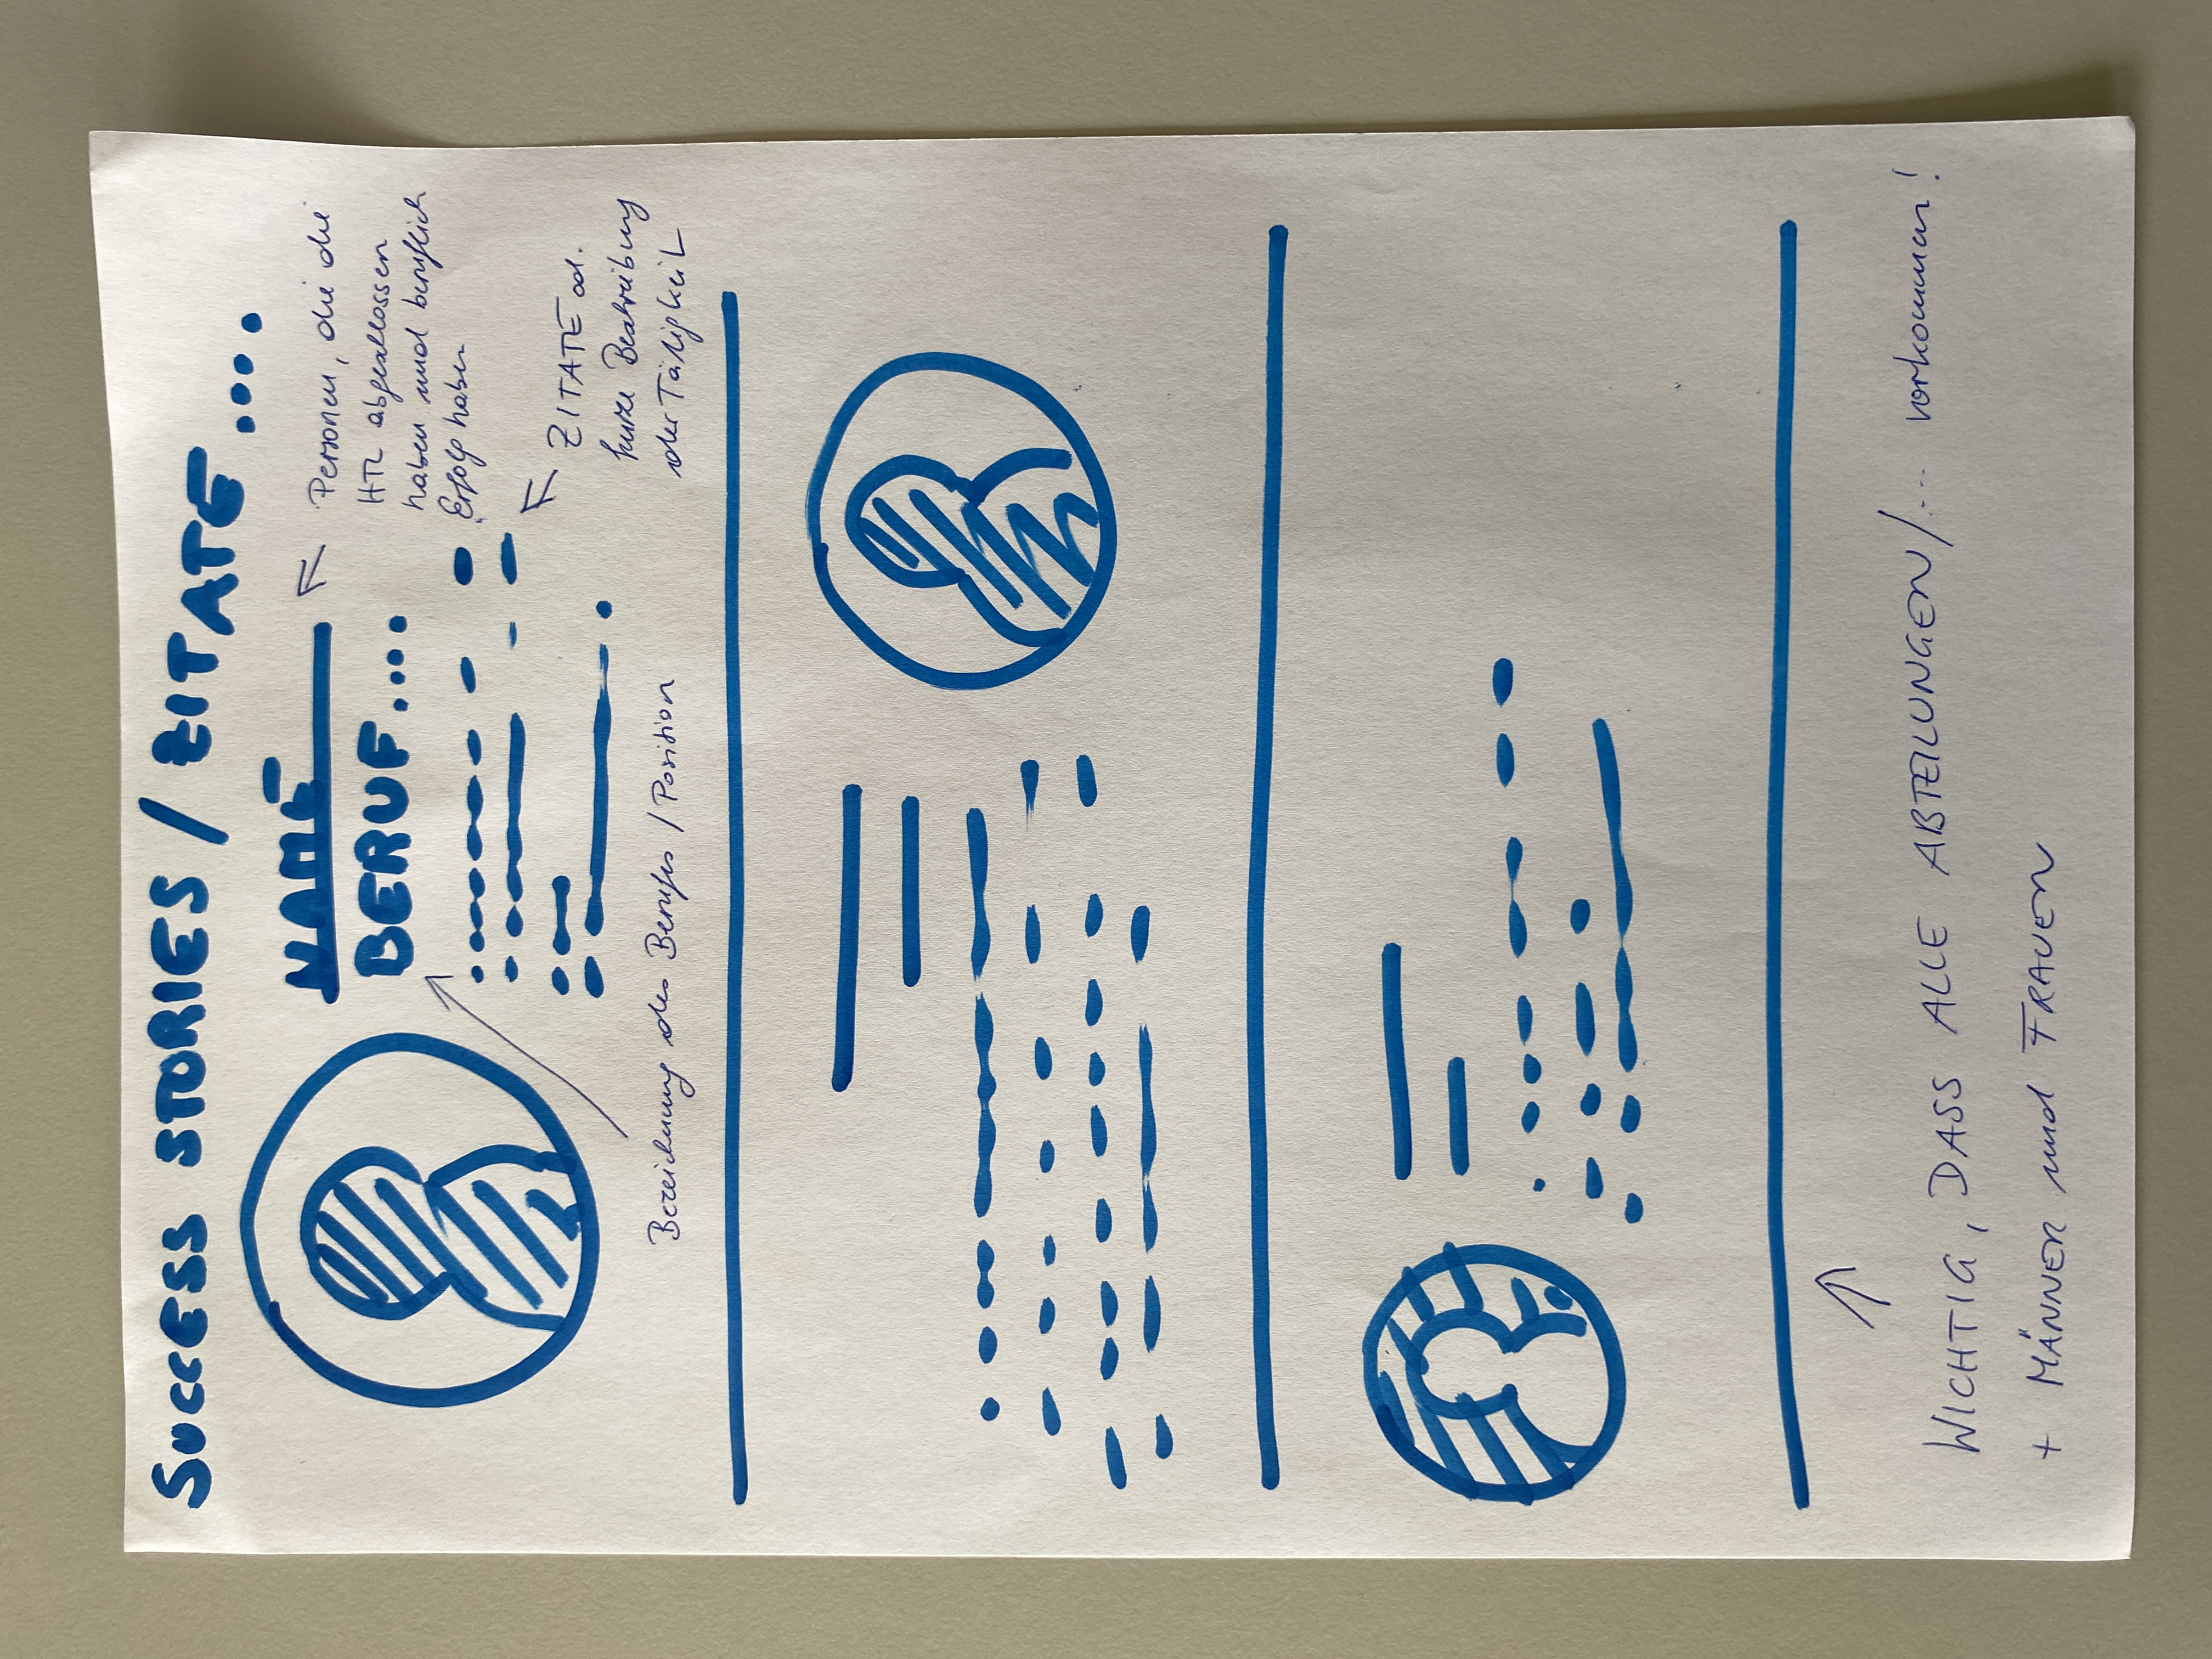
\includegraphics[width=\textwidth, angle=270]{pics/Entwurf_Beispiel_3.JPG}
     \caption{Entwurf 3}
     \label{fig:c}
   \end{subfigure}
   \caption{erste Entwürfe}
   \label{fig:impl:erste_entwuerfe}
 \end{figure}

\section{Entwurf und Usability-Tests}
\setauthor{Angerer Mona}
Nach umfassenden Analysen und Untersuchungen der geeigneten Gestaltungselemente, Effekte und Animationen für die HTL-Website wird unter Anwendung des im Workshop 
erworbenen Wissens und der Designmethoden ein erster Entwurf erstellt. Die Gestaltung wird mithilfe der Plattform Figma in Form eines 
Click-Dummies skizziert. (Siehe Abbildung \ref{fig:impl:figma_entwurf}) Anschließend präsentiert man diesen Entwurf SchülerInnen der ersten und zweiten Klasse der HTL sowie Lehrkräften 
und externen Personen. Diese Form der Testung ermöglicht es, direktes Feedback und Bewertungen zu sammeln, um den Entwurf 
weiter zu verfeinern und optimal an die Bedürfnisse der BenutzerInnen anzupassen. Der Prozess integriert somit gezielt die Perspektiven 
der verschiedenen Zielgruppen, um eine benutzerfreundliche Website zu gewährleisten. 
Die erhaltenen Rückmeldungen bekräftigen die verbesserte Struktur und die aufgewertete Anordnung durch die Reduzierung der Menüpunkte. 
Zudem wird bestätigt, dass die Navigation auf der Benutzeroberfläche merklich vereinfacht wurde. Allerdings werden auch einige Anregungen 
und Kritiken geäußert, darunter die Empfehlung, vermehrt Schülerfotos einzubinden, um die Website persönlicher zu gestalten. Diese Maßnahme 
soll dazu beitragen, ein einladenderes Bild der HTL Leonding zu vermitteln. Auch werden einige Verschiebungen von Inhalt in andere Menüpunkte 
vorgeschlagen, um eine logischere Anordnung sicherzustellen. 
Nach der Implementierung dieser Verbesserungsvorschläge wird der Prozess mehrfach wiederholt, um das Design weiter zu perfektionieren und 
eine optimale Zufriedenheit aller BenutzerInnen sowie eine intuitive Steuerung der Website zu erreichen. 

\begin{figure}
   \begin{minipage}[b]{\linewidth} 
      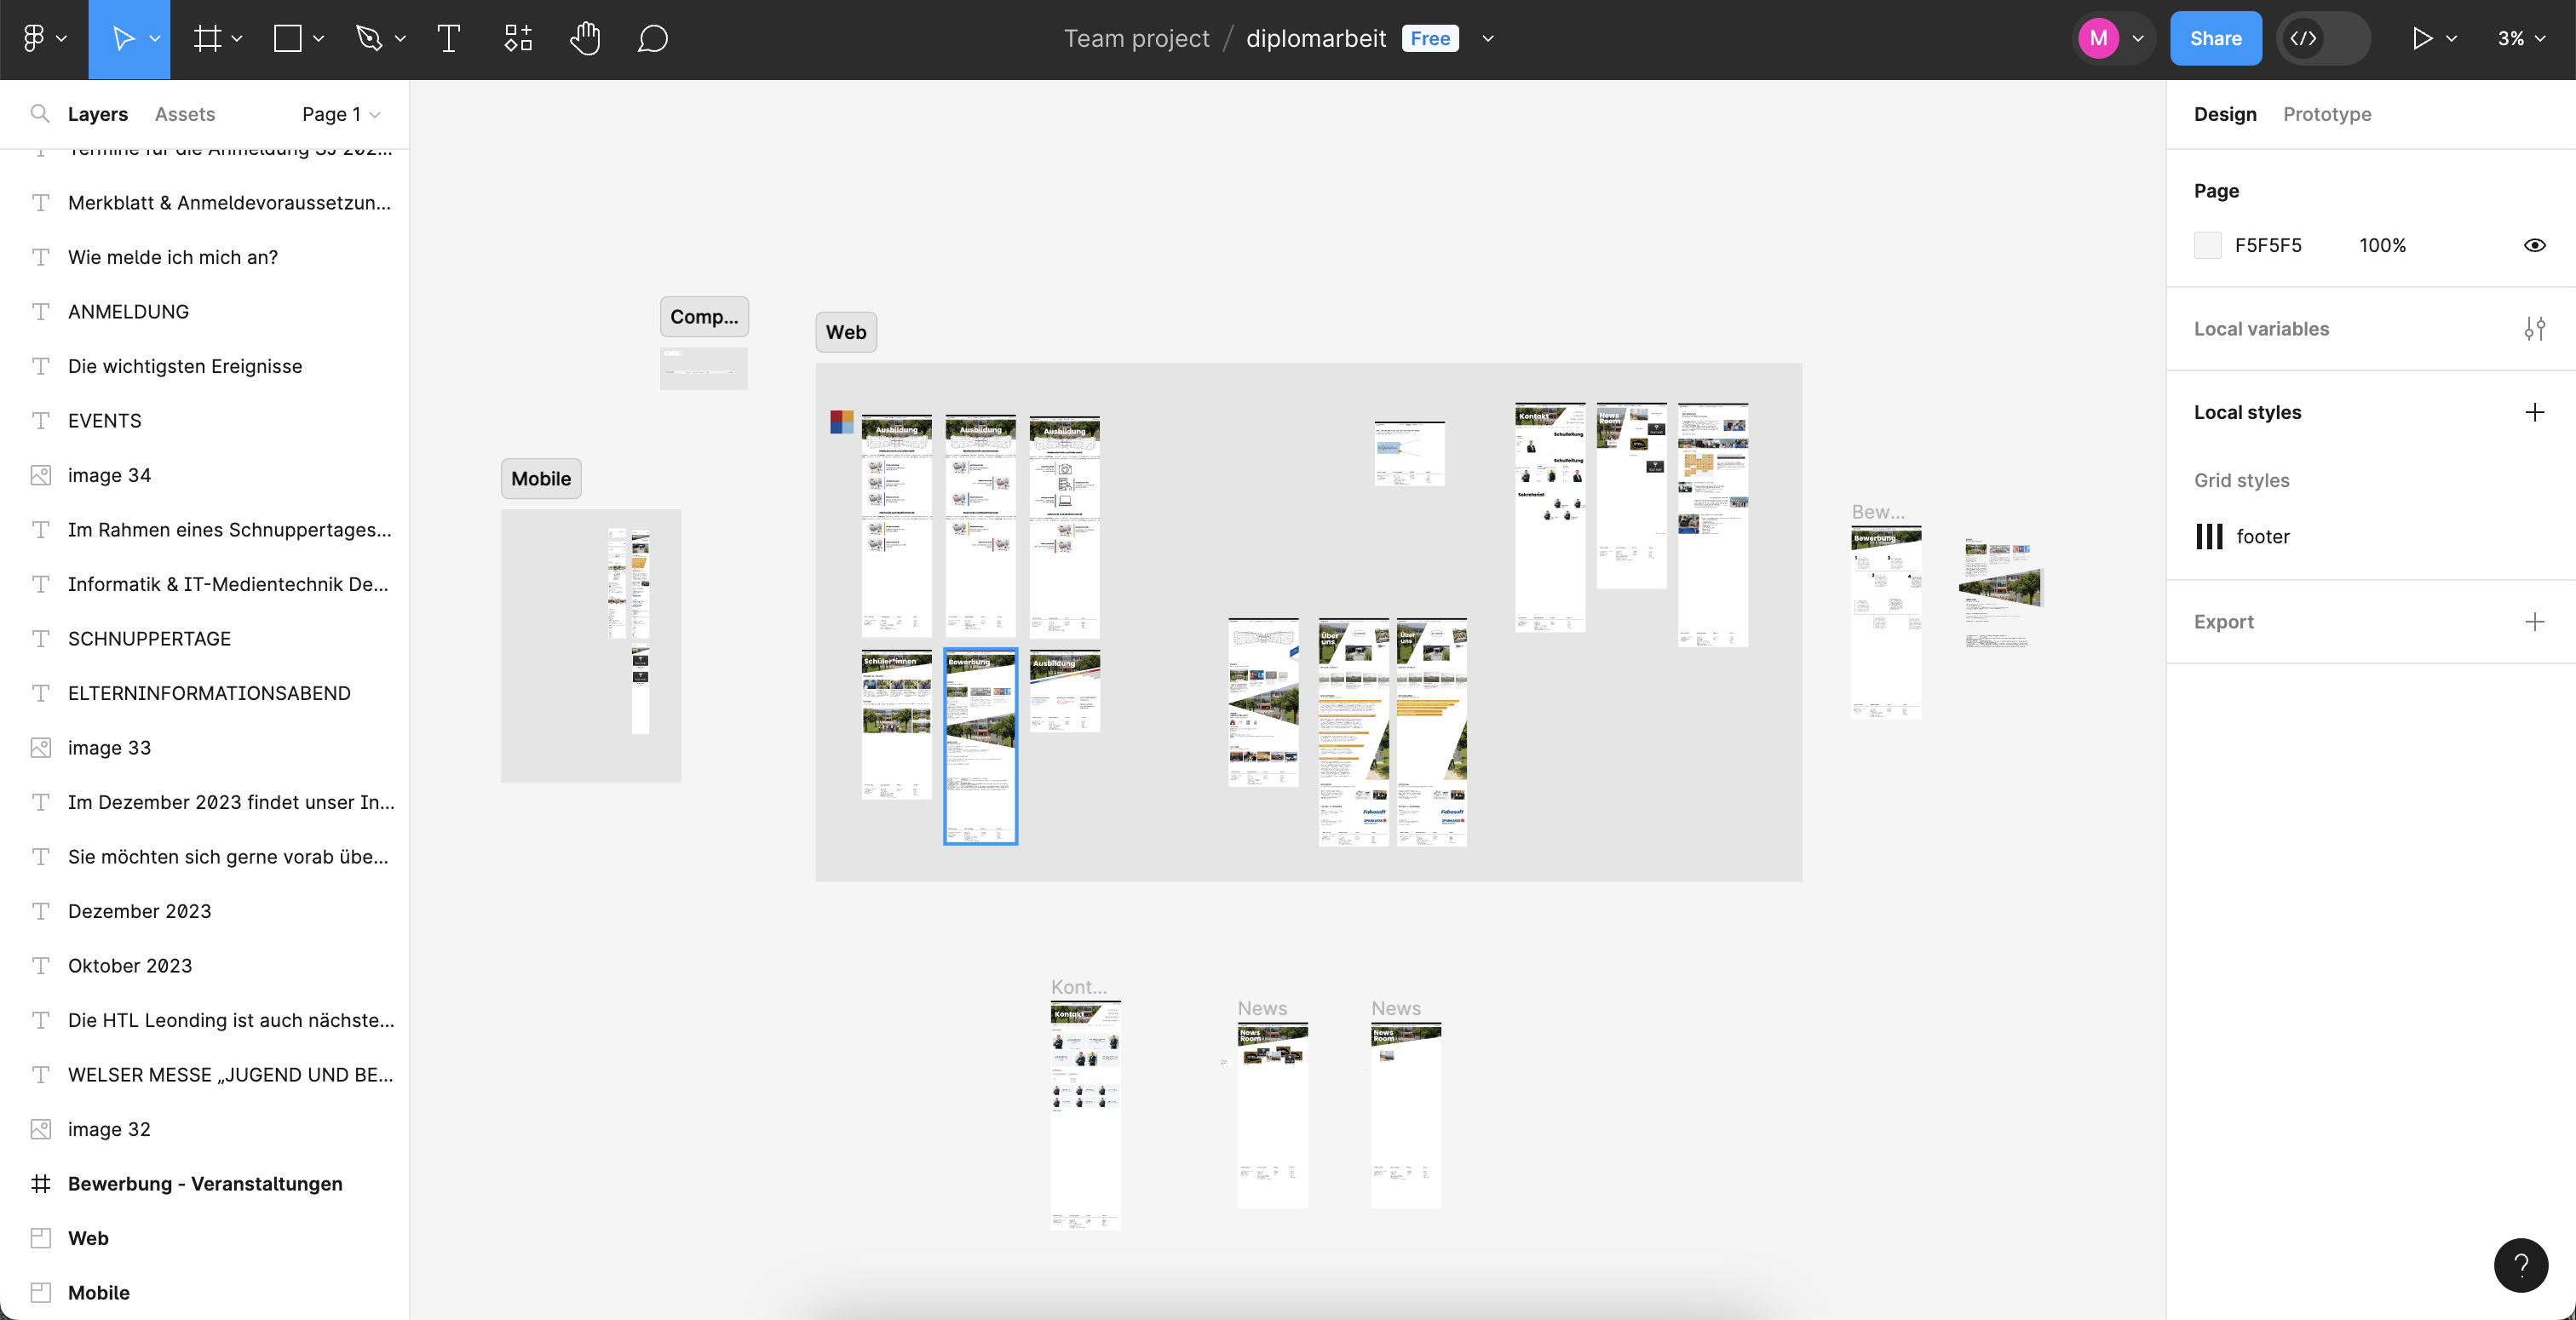
\includegraphics[width=\linewidth]{pics/figma.png}
      \caption{Entwurf mit Figma}
      \label{fig:impl:figma_entwurf}
   \end{minipage}
   \hspace{.05\linewidth}
\end{figure}

\section{Finales Design}
\setauthor{Angerer Mona}
Nachdem der Prozess des Usability-Testings und der Überarbeitungen einige Male durchlaufen
wird, entsteht am Ende ein optimiertes und finales Design. 

Dieses beinhaltet folgende Designelemente und unterscheidet sich in diesen Punkten zu der Gestaltung der bisherigen HTL-Website:


\subsection{Menu und Inhalt}
\setauthor{Angerer Mona}
   Im Vergleich zum alten Menu-Header (Siehe Abbildung \ref{fig:impl:header:alt}) hat der Neue (Siehe Abbildung \ref{fig:impl:header:neu}) statt 7 nur mehr 5 Elemente, um eine sauberere
   Ansicht zu schaffen und Verwirrung in der Navigation zu vermeiden. Die Inhalte aus dem Reiter \glqq News\grqq{} können nun durch einen Link auf der Seite
   \glqq Über uns\glqq{} erreicht werden, die Partnerfirmen stehen nun auf der Startseite. Der Menüpunkt \glqq Schüler:innen\grqq{} ist nun
   aum rechten Bildschirmrand platziert, um die Hauptelemente des Headers erneut zu vermindern und um eine Art \glqq Profil\grqq{}
   oder \glqq Einloggen\glqq{} zu suggestieren. Dort finden sich ebenfalls keine nur für bereits an der HTL Leonding
   lernende Personen, denn dieser Inhalt wurde umfassend in das LeoWiki ausgelagert. Stattdessen findet man unter 
   dem Reiter jetzt die an der Schule angebotenen Programme und SchülerInnenfotos, um einen persönlichen Einblick zu bieten und 
   den Wünschen und Vorschlägen der bei den Usability-Tests befragten Personen nachzugehen.

\begin{figure}
      \centering
      
\includegraphics[scale=0.3]{pics/header_alt.png}
      \caption{alter Header}
      \label{fig:impl:header:alt}
  \end{figure}

  \begin{figure}
   \centering
   
\includegraphics[scale=0.3]{pics/header_neu.png}
   \caption{neuer Header}
   \label{fig:impl:header:neu}
\end{figure}

\subsection{Farben und Formen}
\setauthor{Angerer Mona}
Da die bisherige Website sehr viele Farben beinhaltete, erschien sie überladen und überfordernd.
Nun wird bei der Gestaltung auf viel weiße Fläche gesetzt, die abgesehen von dem Bildmaterial lediglich von kleinen Akzenten 
in den vier Farben der Abteilungen, die auch im Logo vorkommen, und einer fünften Farbe, die eine Mischung der vier 
"HTL-Leonding-Farben" ist, unterbrochen wird. Der Trend zu viel "Whitespace" ist, wie im Kapiel \nameref{sec:Recherche} bereits
behandelt wurde, ein häufig aufkommendes, modernes Designkonzept.

Auch wurde statt auf das starre Block-Design auf mehr Abwechslung und Bewegung in den Formen gesetzt.
So ist das Dreieck eine der wichtigsten Elemente des neuen Webauftritts. Der Grund, weshalt die Wahl 
auf ausgerechnet diese Grundform gefallen ist, liegt in dem Logo der Schule. Dieses besteht aus einem Pfeil,
in dem sich die bereits angesprochenen vier Abteilungsfarben wiederspiegeln. Mittels der verschiedenen
implementierung des Dreiecks auf den unterschiedlichen Seiten der Website spiegeln sich so die Schrägen,
die man bereits im Logo findet, wieder. Auch erscheint der Gesamteindruck
dynamischer und spannender, was zu einer verbesserten User-Experience führt.

\subsection{Dynamik und Bewegung}
\setauthor{Angerer Mona}
Nicht nur die wiederholte Einbringung des nicht-typischen, wandelbaren Elements des Dreiecks
bringt mehr Spannung und dynamik in die Weboberfläche, auch sind viele sich bewegende Objekte auf 
der Website eingebunden. Um allerdings keine Unruhe und Stress in den Benutzern auszulösen, ist dieser
bewegte Content subtil und nicht zu oft angewendet und langsam in seiner Bewegung. Beispiele dafür finden sich 
auf der Seite "Abteilungen", wo sich eine Übersicht der Fächernamen von links nach rechts und umgekehrt
über den Bildschirm bewegt, oder auf den Seiten der einzelnen Abteilungen, wie Beispielsweise "Informatik - SSE", 
wo sich eine Reihe von Bildern, die die Fachrichtung beschreiben, sich vertikal über das Display bewegt.


\subsection{Animationen}
\setauthor{Angerer Mona}
Um das durch den vielen Whitespace erzeugte schlichte Design etwas aufzubrechen, wurde eine Strartanimation,
sowie Animationen für jede Abteilung eingefügt. Die Startanimation, die beim Aufrufen der Website 
abgespielt wird, beginnt mit dem HTL Leonding-Logo mit dem Schriftzug "HTL Leonding next level", geht dazu über dass 
der Schriftzug verschwindet, sich das Logo in die Mitte des Bildschrims bewegt und  in eine vereinfachte Graifk der HTL von oben verwandelt.
In der Schlussposition befindet sich die Grafik der HTL am rechten Bildschirmrand und die 
wichtigsten Events scrollen aus dem Gebäude. 


\begin{spacing}{1}
	\chapter{Animationen}
	\end{spacing}
	Wie im Kapitel Design bereits beschreiben, haben wir um die Website aufzulockern einige Animationen eingebaut. 
In folgendem Abschnitt wird erläutert, mit welchem Verfahren diese ausgewählt wurden, welche Technolgien verwendet wurden und die 
wie die Einbindung auf der Homepage funktioniert.

\section{Auswahl der Animationen und Grafiken} \label{sec:animationen:Aimationen}
\setauthor{Angerer Mona}

Als Grafiken wurde auf simple Darstellungen des Schulgebäudes der HTL Leonding aus verschiedenen Perspektiven gesetzt. 
Eine Abbildung aus der Vogelperspektive (Siehe Abbildung \ref{fig:impl:schule:oben}) ist implementiert in der Startanimation der Homepage, 
eine grafische Verwirklichung der Schule von vorne (Siehe Abbildung \ref{fig:impl:schule:vorne})
ist auf der Unterseite "Abteilungen" zu finden. Insbesondere die zuletzt erwähnte Grafik ist auch in Zukunft, nach Abschluss der Diplomarbeit
für vielseitige Zwecke einsetzbar und kann leicht modifiziert und angepasst werden.

Bei der Auswahl der eingebundenen Animationen wurde großer Wert auf die Benutzerfreundlichkeit und Navigation gelegt.
Deswegen wird beim Aufruf der neuen Homepage direkt mit einer etwa zwei-sekündigen Startanimation begonnen. Diese soll die 
Aufmerksamkeit der User erlangen und einen spannenden Start bieten. Sie startet mit dem HTL Leonding Logo und dem Schriftzug "HTL Leonding next level" und nachdem
das Logo von der linken Seite zur rechten Seite schwebt und der Schriftzug veschwindet verwandelt sich das Logo in eine Grafik des 
HTL Gebäudes aus der Vogelperspektive. Anschließend scrollen die wichtigsten News-Beiträge von rechts aus dem Gebäude. 
Auch wurde für jede Abteilung der HTL eine eigene kleine Animation gefertigt, die die jeweilige Fachriochtung repräsentiert.


\begin{figure}
   \begin{minipage}[b]{.4\linewidth} 
      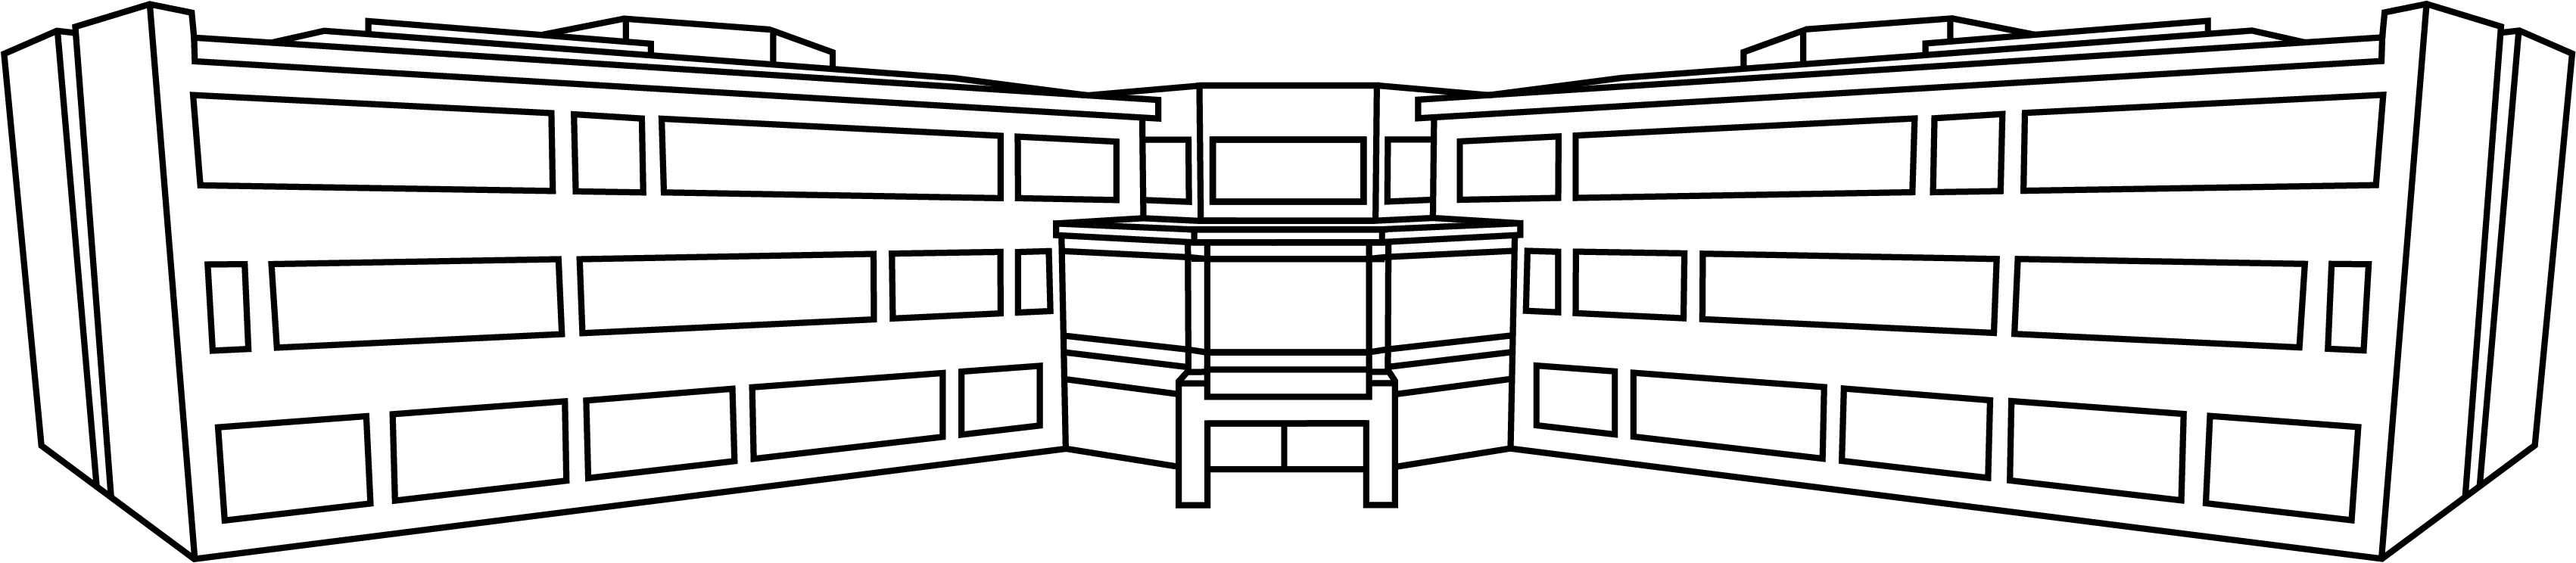
\includegraphics[width=\linewidth]{pics/schule vorne.png}
      \caption{SVG Schule von vorne}
      \label{fig:impl:schule:vorne}
   \end{minipage}
   \hspace{.05\linewidth}
   \begin{minipage}[b]{.4\linewidth}
      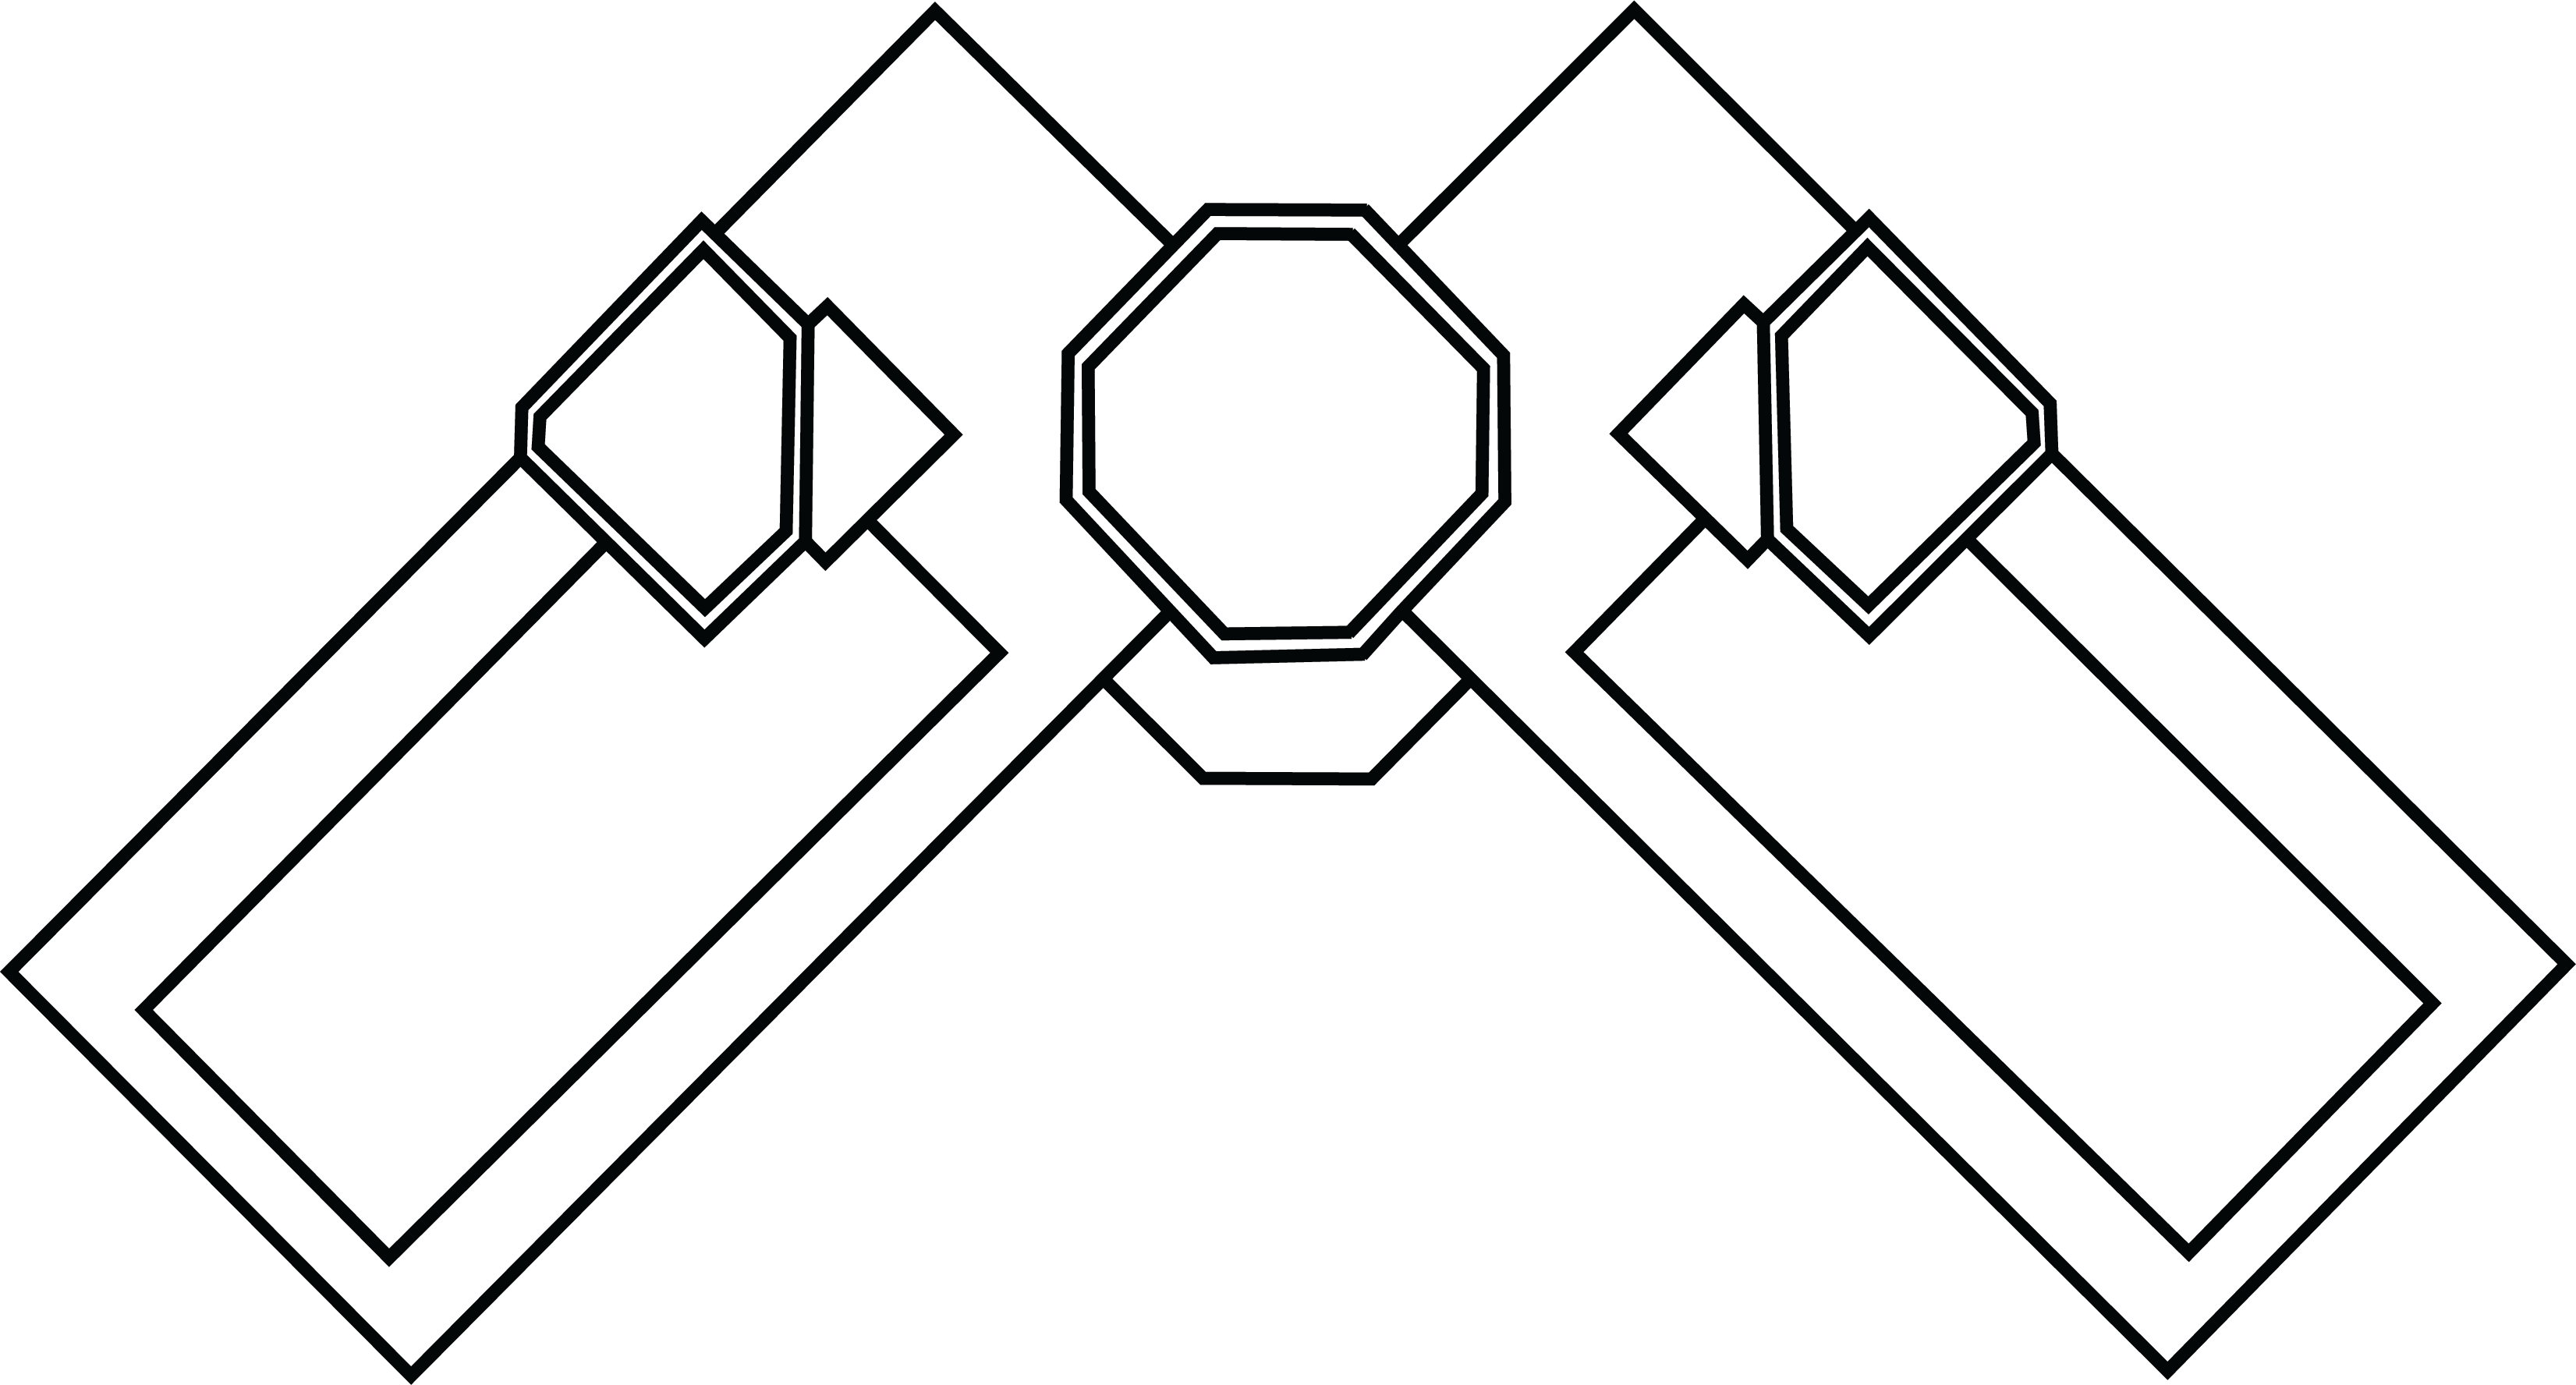
\includegraphics[width=\linewidth]{pics/schule.png}
      \caption{SVG Schule von oben}
      \label{fig:impl:schule:oben}
   \end{minipage}
\end{figure}


\section{Erstellung} \label{sec:animationen:Erstellen}
\setauthor{Angerer Mona}

Für jene Animationen, die nicht von Framer Motion umgesetzt werden, werden die Vektorgrafiken zuerst mittels Adobe Illustrator erstellt. Die Wahl der genutzten Programme zum Aufbereiten der Grafiken und Animationen fiel aus diversen Gründen
auf die Adobe Cloud. Einerseits sind die Anwendungen unter sich optimal kompartibel. Die Zusammenarbeit zwischen den Adobe-Programmen funktioniert 
einwandfrei und ermöglicht so einen optimierten Workflow. Die Vektorbasierte Arbeitsweise garantiert Grafiken ohne Qualitätsverlust bei jeder Skalierung. Auch bitet Illustrator die Möglichkeit, die erstellten Vektorgrafiken direkt als SVG zu exportieren, um anschließénd
in Adobe After Effects diese zu importieren und mit Animationstechniken zu veredeln. In After Effects können verschiedene Animationseffekte, 
Übergänge und Bewegungen hinzugefügt werden, um den Grafiken Leben einzuhauchen und sie dynamischer und ansprechender zu gestalten. 
Dieser Animationsprozess ermöglicht es, komplexe Bewegungen und Interaktionen zu erstellen, die die visuelle Darstellung der Grafiken 
erheblich verbessern.

Nach Abschluss der Animation in After Effects erfolgt der Export der animierten Grafiken im JSON-Format, welches von LottieFiles 
unterstützt wird. LottieFiles wird als Plugin in After Effects hinzugefügt und ist speziell für die Integration von animierten Grafiken in Web- und 
App-Designs entwickelt. Es ermöglicht die nahtlose Einbindung der animierten Grafiken in verschiedene Projekte und Plattformen, 
wobei die hohe Qualität und flüssige Darstellung der Animationen beibehalten wird. Durch die Verwendung von LottieFiles können die 
animierten Grafiken effizient in die Website integriert werden, ohne die Ladezeiten oder die Leistung der Website zu beeinträchtigen.


\section{Einbindung} \label{sec:animationen:Einbindung}
\setauthor{Angerer Mona}

\subsection{Framer Motion}
\setauthor{Mona Angerer}
Für die Umsetzung aller Animationen mit Ausnahme der SVG-Animationen auf der Website wurde das Animationsframework für React
Framer Motion ausgewählt. Es bietet eine leistungsstarke und flexible Lösung für 
die Erstellung von dynamischen und ansprechenden Animationen, die den HTML- und CSS-Code der Website betreffen.

Im Gegensatz zu herkömmlichen CSS-Animationen bietet Framer Motion ein breites Spektrum an fortschrittlichen 
Animationstechniken und -funktionen, die weit über einfache Transitions und Effekte hinausgehen. Eines der herausragenden 
Merkmale dieses Frameworks sind die Layout-Animationen, die es ermöglichen, komplexe seitenübergreifende Transformationen zu realisieren. 
Diese Layout-Animationen bieten die Möglichkeit, den Inhalt und die Struktur der Website dynamisch und ansprechend zu gestalten, 
wodurch ein flüssiges und nahtloses Benutzererlebnis geschaffen wird.

Darüber hinaus bietet Framer Motion spezialisierte Funktionen für Load- und Unload-Animationen. Diese sind darauf 
ausgerichtet, das Laden und Entladen des DOM (Document Object Model) zu animieren, um fließende und eindrucksvolle Seitenübergänge 
zu ermöglichen. Dies trägt maßgeblich zur Verbesserung der visuellen Darstellung und Benutzerfreundlichkeit der Website bei.

Die vielseitigen und erweiterten Funktionen von Framer Motion ermöglichen es, die Animationen und Interaktionen auf der 
Website gezielt und präzise zu steuern. Sie bieten eine hohe Flexibilität und Anpassungsfähigkeit, wodurch die individuellen 
 Animationseffekte leicht umgesetzt werden können.

 \subsection{Lottie}
\setauthor{Angerer Mona}
Als zentrales SVG-Animationsframework für die Implementierung der animierten SVG-Grafiken auf der Website wird Lottie verwendet. 
Dieses Framework bietet eine leistungsstarke Lösung für die Darstellung von komplexen und ansprechenden Animationen direkt im Webbrowser, 
ohne die Ladezeiten oder die Performance der Website negativ zu beeinflussen.

Nachdem Lottie als Plugin in After Effects hinzugefügt wird (zu finden in After Effects siehe Abbildung \ref{fig:impl:plugin:lottie}), können im Exportprozess aus Adobe After Effects die Animationen speziell als Lottie JSON 
exportiert, wodurch eine nahtlose und fehlerfreie Kompatibilität zwischen den beiden Programmen garantiert wird. Die gewonnenen JSON-Files 
können anschließend problemlos in die 
Website eingebunden werden.

\begin{figure}
   \begin{minipage}[b]{.4\linewidth} 
      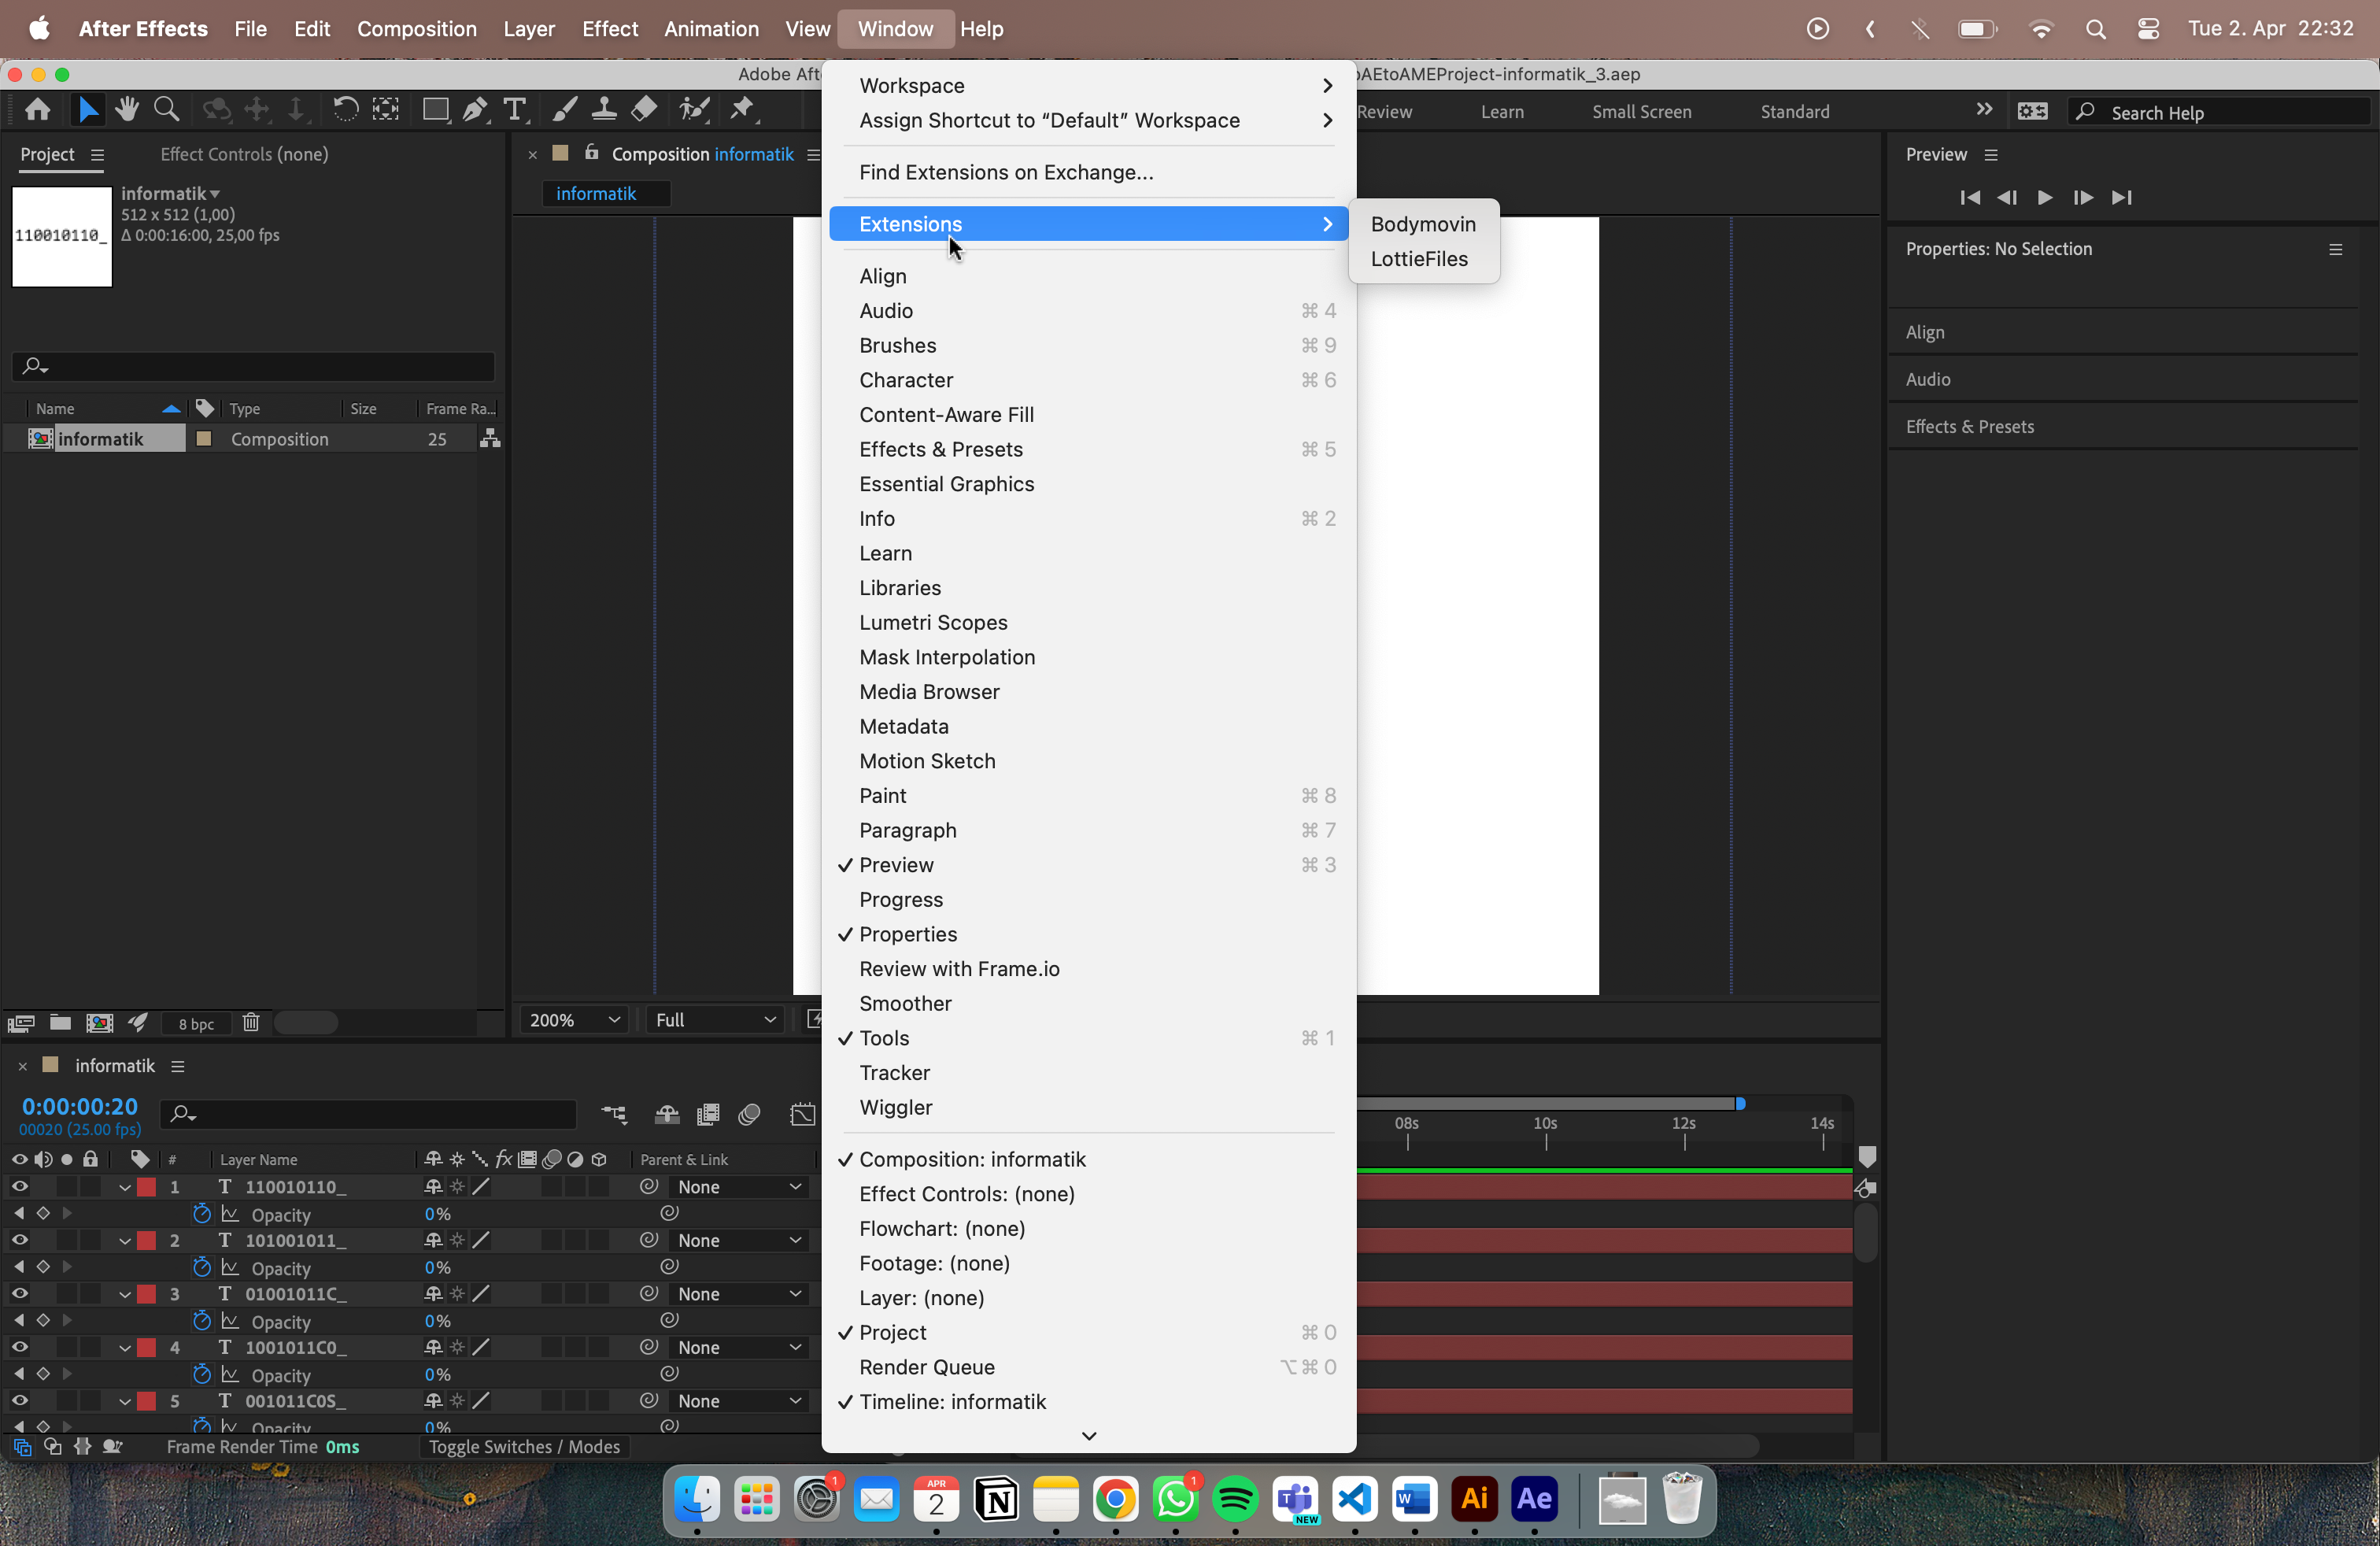
\includegraphics[width=\linewidth]{pics/plugin lottie.png}
      \caption{Lottie als Plugin in After Effects}
      \label{fig:impl:plugin:lottie}
   \end{minipage}
\end{figure}

Nach dem Export erfolgt die Implementierung der animierten Grafiken im Code durch die Einbindung dieser JSON-Dateien 
in den Lottie Player. Der Lottie Player ist ein spezialisiertes JavaScript-Plugin, das die Darstellung der Lottie JSON-Dateien im 
Webbrowser steuert. Durch diese Kombination werden alle übrigen Animationen, die nicht durch Framer Motion oder andere Technologien 
gesteuert werden können, effizient und zuverlässig durch Lottie gesteuert.

Beschreibene Vorgehensweise bietet den Vorteil, dass komplexe und detailreiche Animationen, die mit Adobe After Effects erstellt wurden, 
direkt und ohne Qualitätsverlust auf der Website dargestellt werden können. Die Verwendung von Lottie bietet eine höhere 
Flexibilität und Anpassungsfähigkeit der Animationen, da sie leicht aktualisiert oder modifiziert werden können, ohne den gesamten Code 
oder die Website neu zu laden.


\section{Schwierigkeiten} \label{sec:animationen:Schwierigkeiten}
\setauthor{Angerer Mona}

Als eine der größten Schwierigkeiten im Punkt Animationen und Grafik bot die Unstimmigkeit und Vielzahl der Ideen. Viele Male wurden Animationen
erstellt, die es im Endeffekt doch nicht auf die Endversion der Homepage geschafft haben, da sich neue und bessere Ideen boten. Dies stellte sich 
als große zeitliche Hürde da und forderte viele Arbeitsstunden.
Auch bereitete der Export der Animationen und die anschließende Einbindung auf der Website einige Schwierigkeiten. 
Da die Ursprungsidee, die Animationen als Videodatein einzubinden aufrgund resultierender hoher Ladezeiten und eingeschreänkter Interaktivität
schnell verworfen wurde, lag die Lösung, JSON-Animationen zu benutzen, nahe.
Es gab zwischenzeitliche Probleme, als versucht wurde die Animaitonen aus After Effects mittels Bodymovin (ein Plugin für Adobe After Effects, das es ermöglicht, 
Animationen aus After Effects-Projekten in das JSON-Format zu exportieren) zu rendern, da einige Bilddatein von dem Plugin nicht richtig interpretiert wurden.



\begin{spacing}{1}
\chapter{Technologien}\label{chapter:tech}
\end{spacing}
\section{Storyblok}
\lipsum[5-12]


\begin{spacing}{1}
\chapter{Umsetzung}\label{chapter:implementation}
\end{spacing}


\section{Storyblok}
\setauthor{Peter Klose}

In Storyblok muss zuallererst die gewollte Struktur der Webseite widergespiegelt werden. Dies wird im Bereich 'Content' gemacht. 
Für Pfade mit Unterseiten werden Ordner erstellt und die restlichen Seiten  als 'Page', 'Branch' oder 'Article' definiert.
Die Content-Gestaltung und Festlegung findet dann in diesen 3 Typen statt. 


\subsection{Storyblok API}

\subsection{Bausteine der Webseite}
Wie der Name schon andeutet, handelt vieles in diesem headless CMS von Blöcken. Diese haben Variablen, welche dann im Editor mit Content befüllt werden können. 
Einen Überblick über alle verfügbaren Blöcke hat man in der Block library. Dort kann man auch neue Blöcke erstellen. In der finalen Version der Webseite sind 41 Blöcke zu finden. 

All unsere Blöcke enstprechen der selben Namensschreibweise. Dabei wird die Snake case Schreibweise verwendet, diese beginnen immer klein und mehrere Worte trennt ein \textunderscore  als Beispiel 'default\textunderscore component'.

In einem Block gibt es dann eine Ansammlung von Feldern, dabei gibt es mehrere zur Auswahl:

% https://www.storyblok.com/docs/schema-configuration#field-types

\begin{longtable}[c]{|l|p{10cm}|}
    \caption{Field Types, die von Storyblok bereitgestellt werden}
    \label{tab:beispiel} \\
    \hline
    \textbf{Feldname} & \textbf{Beschreibung} \\
    \hline
    \endhead
    %
    \hline
    \endfoot
    %
    Blocks & Weitere Blöcke können hinzugefügt werden. \\
    \hline
    Text & Einfaches einzeiliges Textfeld \\
    \hline
    Textarea & Mehrzeiliges Textfeld ohne Formatierung \\
    \hline
    Richtext & Mehrzeiliges Textfeld mit Formatierungsmöglichkeiten (JSON Format) \\
    \hline
    Markdown & Mehrzeiliges Textfeld mit Formatierungsmöglichkeiten (Markdown Format) \\
    \hline
    Number & Nummernfeld ohne Formatierung \\
    \hline
    Date/Time & Datum und Uhrzeit - Picker \\
    \hline
    Boolean & Checkbox - true/false \\
    \hline
    Multi-Options & Liste von Schlüssel-Wert-Paaren, die konfigurierbar sind. Entweder hartcodiert, als externes JSON oder als Datenbank. Mehrere Werte sind auswählbar \\
    \hline
    Single-Option & Liste von Schlüssel-Wert-Paaren, die konfigurierbar sind. Entweder hartcodiert, als externes JSON oder als Datenbank. Kein oder ein Werte sind auswählbar \\
    \hline
    Asset & Fileauswahl, die in den Typen limitiert werden kann (nur Images, Videos, Audio, Textdokumente) aber ansonsten alle Typen annimmt. \\
    \hline
    Multi-Assets & Fileauswahl, die in den Typen limitiert werden kann (nur Images, Videos, Audio, Textdokumente) aber ansonsten alle Typen annimmt. Mehrere Files können hier gleichzeitig ausgewählt werden. \\
    \hline
    Link & Link auf eine Unterseite aus Storyblok oder als extere URL \\
    \hline
    Table & In der größe Formatierbare Tabelle, keine Textformatierung möglich \\
    \hline
    Group & Gruppierungs Folder für die Attribute\\
    \hline
    Image(old) & Veraltete Option Bilder einzubinden - Asset sollte nun verwendet werden \\
    \hline
    File(old) & Veraltete Option Files einzubinden - Asset sollte nun verwendet werden \\
    \hline
    Plugin & Zugriff auf externe Storyblok-Pugins - UI UX differenziert mit jedem Plugin \\
    \hline
\end{longtable}

All diese Attribute haben ein Bearbeitungsfenster, welches von oben nach unten mindestens den Typen, Darstellungsnamen, Technischen Namen, Checkbox - Notwendig, Checkbox - Übersetzbar und Beschreibungsfeld bietet.

Die 2 Wichtigsten sind aber die beiden Checkboxen. Sie ermöglichen uns sicherzustellen, dass der Wert gesetzt werden muss (Checkbox - Notwendig) und dass man ihn falls Notwendig übersetzten kann (Checkbox - Übersetzbar). 

Nachstehen werden diese beiden Checkboxen mit den in Klammern stehenden englischen Buchstaben angezeigt.

\subsubsection*{Page}
Der Page-Block war schon vorgefertigt von Storyblok und wurde genau so übernommen.
Er ist sehr simpel aufgebaut das einzige Attribut, welches er beinhaltet ist body ein Blocks Element.

\subsubsection*{Article}
Article ist der Blok, welcher für News, Projekte, Clubs bzw. Events benutzt wird. 
Wie Page ist er ein Root Level Block, er besitzt jedoch keinen dynamischen body sondern nur folgende Attribute

\begin{longtable}[c]{p{3cm}ccp{6cm}}
    \caption{Attribute des Article Blocks}
    \label{tab:article}\\
    \toprule
    \textbf{Attribute} & \textbf{R} & \textbf{T} & \textbf{Beschreibung} \\
    \midrule
    \endhead
    %
    \endfoot
    %
        headline & \checkmark & & Überschrift des Newsbeitrags oder Events \\
        subline & & \checkmark & Unterüberschrift \\
        type & \checkmark & & Typ des Artikels: News, Event, Projekt, Club \\
        allocate & & & Zugeordnete Abteilung, mitunter auch Allgemein, Sport oder Reisen \\
        date & \checkmark & & Erstellungsdatum, Datum des Events \\
        content & \checkmark & & Formatierter Text \\
        image & \checkmark & & Titelbild für diesen Beitrag \\
        assets & & & Weitere Medien \\
        subpage\_enabled & & & Soll ein Link zur vollen Seite dieses Beitrags angezeigt werden \\
\end{longtable}

\subsubsection*{Branch}
Branch spiegelt unsere Abteilungen wieder, er bietet wie Page einen body an Blocks und weitere wichtige Attribute zur richtigen Darstellung der Abteilungen sind:

\begin{longtable}[c]{p{3cm}ccp{6cm}}
    \caption{Attribute des Branch Blocks}
    \label{tab:article}\\
    \toprule
    \textbf{Attribute} & \textbf{R} & \textbf{T} & \textbf{Beschreibung} \\
    \midrule
    \endhead
    %
    \endfoot
    %
    headline & \checkmark & \checkmark & Abteilungsname \\
    subline & & \checkmark & Kurzbeschreibung der Abteilung \\
    allocate & & & Zugeordnete Abteilung \\
    imagevideo & & & Link zum YouTube-Video der Abteilung \\
    folder & & & Hinterlegter PDF-Folder der Abteilung \\
    description & & & Beschreibung der Abteilung \\
\end{longtable}

\subsubsection*{All Articles }
All Articles ist in Storyblok ein relativ simpler Block, er dient dazu alle Articles die zu einer bestimmten Kategorie gehören anzuzeigen.  

\begin{longtable}[c]{p{3cm}ccp{6cm}}
    \caption{Attribute des All Articles Blocks}
    \label{tab:article}\\
    \toprule
    \textbf{Attribute} & \textbf{R} & \textbf{T} & \textbf{Beschreibung} \\
    \midrule
    \endhead
    %
    \endfoot
    %
    headline & \checkmark & \checkmark & Überschrift \\
    type & \checkmark & & Article Kategorie Auswahl (News,Events,Projekte,Clubs) \\
    filter & & & Filtermöglichkeit der Articles (default: false) \\
\end{longtable}

\subsubsection*{Basic Slider}
Basic Slider ist wie der Name schon sagt ein einfacher Slider, welcher mit einem Mouse drag bedient wird. Da dieser aber nicht perfekt in unser UI,UX-Design passt könnte es sein dass er durch den Scroll Slider ersetzt wird.  

\begin{longtable}[c]{p{3cm}ccp{6cm}}
    \caption{Attribute des Basic Slider Blocks}
    \label{tab:blockname}\\
    \toprule
    \textbf{Attribute} & \textbf{R} & \textbf{T} & \textbf{Beschreibung} \\
    \midrule
    \endhead
    %
    \endfoot
    %
    headline & \checkmark & \checkmark & Überschrift \\
    content & \checkmark & & Mindestens 3 Iframe Container sind notwendig, andere Blocks sind nicht erlaubt \\
\end{longtable}

\subsubsection*{Classes}
Classes stellt die Struktur für die Darstellung der Klassen an der HTL dar. Es handelt sich also um eine Abgeschlossene Sektion als Blok in dem Content sind nur Class Entry Blocks erlaubt.

\begin{longtable}[c]{p{3cm}ccp{6cm}}
    \caption{Attribute des Classes Blocks}
    \label{tab:blockname}\\
    \toprule
    \textbf{Attribute} & \textbf{R} & \textbf{T} & \textbf{Beschreibung} \\
    \midrule
    \endhead
    %
    \endfoot
    %
    headline & \checkmark & \checkmark & Überschrift \\
    content & \checkmark & & Beliebige Anzahl von Class Entry Blocks \\
\end{longtable}

\subsubsection*{Classes Entry}
Classes Entry stellt wirklich genau eine Klasse dar. Gedacht währe als Foto ein Klassenfoto.  

\begin{longtable}[c]{p{3cm}ccp{6cm}}
    \caption{Attribute des Classes Entry Blocks}
    \label{tab:blockname}\\
    \toprule
    \textbf{Attribute} & \textbf{R} & \textbf{T} & \textbf{Beschreibung} \\
    \midrule
    \endhead
    %
    \endfoot
    %
    classname & \checkmark & & Name der Klasse \\
    img & \checkmark & & Klassenfoto der Klasse als Datei (nur Bilder erlaubt) \\
    headofclass & & & Klassenvorstand der Klasse \\
\end{longtable}

\subsubsection*{Custom Image}
Custom Image dient als Grundlage falls im Frontend spezielle Anforderungen an ein Bild gestellt sind. Wie in Über Uns, wo die Broschüre gedreht ist.  

\begin{longtable}[c]{p{3cm}ccp{6cm}}
    \caption{Attribute des Custom Image Blocks}
    \label{tab:blockname}\\
    \toprule
    \textbf{Attribute} & \textbf{R} & \textbf{T} & \textbf{Beschreibung} \\
    \midrule
    \endhead
    %
    \endfoot
    %
    image & \checkmark & & Darzustellende Bilddatei \\
    type & & & Single-Select Liste der speziellen Anforderungen, wie es dargestellt werden soll \\
\end{longtable}

\subsubsection*{Custom Link}
Custom Link dient dazu alle Links die existieren gleich zu gestalten. Obwohl ein Link-Attribut in Storyblok existiert haben wir uns nicht dafür ausgesprochen, weil es keine Möglichkeit gibt Symbole oder andere Spezielle Styles zu hinterlegen.  

\begin{longtable}[c]{p{3cm}ccp{6cm}}
    \caption{Attribute des Custom Link Blocks}
    \label{tab:blockname}\\
    \toprule
    \textbf{Attribute} & \textbf{R} & \textbf{T} & \textbf{Beschreibung} \\
    \midrule
    \endhead
    %
    \endfoot
    %
    link & \checkmark & & Link zu internen oder externen Medien bzw. Seiten \\
    symbol & & & Auswählbare Symbole, die vor dem Link angezeigt werden \\
    display\textunderscore name & \checkmark & \checkmark & Anzeigename des Links \\
\end{longtable}

\subsubsection*{Designable Table}
Storyblok bietet ein Plugin, welches es ermöglicht Tabellen darzustellen. Bei diesem Plugin ist es jedoch nicht möglich einen designten Body (fetter und farbiger Text) einzufügen. Aus diesem Grund wurde ein eigener Blok erstellt, welcher diese Probleme beseitigt.

\begin{longtable}[c]{p{3cm}ccp{6cm}}
    \caption{Attribute des Designable Table Blocks}
    \label{tab:blockname}\\
    \toprule
    \textbf{Attribute} & \textbf{R} & \textbf{T} & \textbf{Beschreibung} \\
    \midrule
    \endhead
    %
    \endfoot
    %
    headline & & \checkmark & Überschrift \\
    columns & \checkmark & & Anzahl der gewünschten Spalten \\
    header & \checkmark & & Der 'Table Row' Block wird vorgesehen, die Menge ist dabei auf 1 limitiert \\
    body & \checkmark & $\geq 1$ & Mindestens ein 'Table Row' Block wird vorgesehen \\
\end{longtable}

\subsubsection*{Table Row}
Der Table Row Block, stellt eine Zeile der Tabelle dar. Aus diesem Grund wurde bei den Attributen des Blocks nur ein value hinterlegt, welches wieder 'Blocks' Element ist. Bei diesem ist die Blockauswahl auf 'Table Value' Limitiert.

\subsubsection*{Table Value}
Der 'Table Value' Block wurde so konfiguriert, sodass die einzige Eingabe ein Richtext-Element ist. Durch dieses wird eine komplette Formatierung gewährleistet.

\subsubsection*{Faq Collection}
Um die häufig gestellen Fragen und Anworten darstellen zu können wurde eine FAQ Ansammlung erstellt.

\begin{longtable}[c]{p{3cm}ccp{6cm}}
    \caption{Attribute des Faq Collection Blocks}
    \label{tab:blockname}\\
    \toprule
    \textbf{Attribute} & \textbf{R} & \textbf{T} & \textbf{Beschreibung} \\
    \midrule
    \endhead
    %
    \endfoot
    %
    headline & \checkmark & \checkmark & Überschrift \\
    description & & & Zusätzliche Beschreibung als Richtext \\
    faqs & \checkmark & & Beliebige Anzahl von FAQ-Element Blocks \\
\end{longtable}

\subsubsection*{Faq Element}
Faq Element dient wiederum nur zur Befüllung der FAQ Collection.

\begin{longtable}[c]{p{3cm}ccp{6cm}}
    \caption{Attribute des Faq Element Blocks}
    \label{tab:blockname}\\
    \toprule
    \textbf{Attribute} & \textbf{R} & \textbf{T} & \textbf{Beschreibung} \\
    \midrule
    \endhead
    %
    \endfoot
    %
    question & \checkmark & \checkmark & Einfacher Text für die Frage \\
    answer & \checkmark & \checkmark & Richtext für eine formatierte Antwort \\
    video & & & Link zur Antwort-Video von Direktor DI Richard Kainerstorfer \\
    show\textunderscore video & & & Boolescher Wert ob das Video angezeigt werden soll oder nicht (default: false) \\
\end{longtable}

\subsubsection*{Footer}
Footer ist der Block, wie der Name schon sagt, der den Footer der Webseite wiederspiegelt. Seine Attribute beinhalten nur footer\textunderscore bg - ein Bild welches zu späziellen Anlässen als Hintergrund verwendet werden kann und columns eine Ansammlung von Footer Col Blöcken.

\subsubsection*{Footer Col}
Der Footer Col Block ist eine Spalte des Footers - hierbei wurde eine Überschift der spalte (headline) und eine Ansammlung an Weiterführenden Links (links) für die Umsetzung eingerichtet.

\subsubsection*{Grid}
Der Grid Block wurde so eingerichtet, sodass alle gängigen Grids Konfiguriert werden konnen. Dafür wurden einige Attribute festgelegt.

\begin{longtable}[c]{p{3cm}ccp{6cm}}
    \caption{Attribute des Grid Blocks}
    \label{tab:blockname}\\
    \toprule
    \textbf{Attribute} & \textbf{R} & \textbf{T} & \textbf{Beschreibung} \\
    \midrule
    \endhead
    %
    \endfoot
    %
    content & \checkmark & & Ansammlung von Blöcken, die einen definierten oder konfigurierbaren Column Span haben \\
    columns & \checkmark & & Minimale Anzahl der Spalten \\
    mediumcolumns & & & Spaltenanzahl ab einer Breite von 768px \\
    largecolumns & & & Spaltenanzahl ab einer Breite von 1024px \\
    max\_w & & & Maximale Breite des Grids \\
    width & & & Definiert als Column Span (nur notwendig, wenn ein Grid in einem anderen Grid verwendet wird) \\
\end{longtable}

\subsubsection*{Grid Item}
Grid Item bietet den Content für das Grid um vielseitig einsetzbar zu sein sind viele Konfigurationen möglich.
\begin{longtable}[c]{p{3cm}ccp{6cm}}
    \caption{Attribute des Grid Item Blocks}
    \label{tab:blockname}\\
    \toprule
    \textbf{Attribute} & \textbf{R} & \textbf{T} & \textbf{Beschreibung} \\
    \midrule
    \endhead
    %
    \endfoot
    %
    headline & & \checkmark & Überschrift \\
    subline & & \checkmark & Unterüberschrift \\
    content & & \checkmark & Formatierbarer Text als Richtext \\
    width & & & Festlegung des Column Span des Elements \\
    type & & & Definiert den Stil des Elements (Ausbildung, Hochformat, Querformat) \\
    content\_type & & & Definiert, ob Main\_Image oder eine Animation angezeigt wird \\
    animation & & & Auswahl aus den verschiedenen Animationen der Abteilungen - nur verfügbar, wenn content\_type = animation \\
    main\_image & & & Hauptbild für dieses Grid-Item \\
    image\_right & & & Boolescher Wert (default: false) \\
    link & & & Link, auf den das gesamte Element verweist \\
    sub\_images & & & Ansammlung von mehreren zusätzlichen Bildern \\
    allocate & & & Zuordnung zu den Abteilungen \\
\end{longtable}

\subsubsection*{Headline}
Headline bietet die Möglichkeit Blöcke ohne Überschrift oder Abschnitten eine passende Überschrift zu geben. Sie beinhaltet nur die Attribute headline und no\_spacing\_y.

\subsubsection*{Hero}
Hero definiert die Oberste Sektion in all unseren Seiten ausgenommen der Startseite. Die Besonderheit ist das Schräge bild und der zusätzlich mögliche Content.
\begin{longtable}[c]{p{3cm}ccp{6cm}}
    \caption{Attribute des Hero Blocks}
    \label{tab:hero}\\
    \toprule
    \textbf{Attribute} & \textbf{R} & \textbf{T} & \textbf{Beschreibung} \\
    \midrule
    \endhead
    %
    \endfoot
    %
    headline & \checkmark & \checkmark & Große Überschrift \\
    background\_image & \checkmark & & Bild, welches hinter der Überschrift liegt \\
    type & \checkmark & & Definiert das Aussehen des Hero Elements \\
    height & \checkmark & & Setzt die Höhe der Sektion \\
    fixed & & & Boolescher Wert, der die Position auf absolut setzt (default: false) \\
    hero\_features & \checkmark & & Blocks Attribut, das mit den Hero Feature Blöcken befüllt werden kann \\
    additional\_content & & & Wird nur bei News, Events und weiteren verwendet, der gesamte Inhalt befindet sich somit in der Hero Component \\
\end{longtable}

\subsubsection*{Hero Feature}
Zusätzliche Information kann hiermit neben dem Hero Block angezeigt werden. Dieser ist wieder konfigurierbar um verschiedene Styles und Funktionen zu ermöglichen.
\begin{longtable}[c]{p{3cm}ccp{6cm}}
    \caption{Attribute des Hero Feature Blocks}
    \label{tab:blockname}\\
    \toprule
    \textbf{Attribute} & \textbf{R} & \textbf{T} & \textbf{Beschreibung} \\
    \midrule
    \endhead
    %
    \endfoot
    %
    symbol & & & Bietet eine Auswahl an Symbolen an, die davor angezeigt werden können \\
    type & \checkmark & & Definiert die Darstellung entweder groß oder klein \\
    text & & & Dargestellter Text \\
    link & & & Falls notwendig, kann ein weiterführender Link angegeben werden \\
\end{longtable}

\subsubsection*{IFrame Container}
Um IFrames per Storyblok einbauen zu können wurde der IFrame Container Block erstellt, dieser bietet durch den Link die Möglichkeit beliebige IFrames wie Videos, Maps oder Ähnliches einzubinden. 
\begin{longtable}[c]{p{3cm}ccp{6cm}}
    \caption{Attribute des IFrame Container Blocks}
    \label{tab:blockname}\\
    \toprule
    \textbf{Attribute} & \textbf{R} & \textbf{T} & \textbf{Beschreibung} \\
    \midrule
    \endhead
    %
    \endfoot
    %
    headline & \checkmark & \checkmark & Überschrift \\
    iframe\_content & \checkmark & & Link zu dem einzubindenden IFrame \\
    links & & & Ansammlung von Custom Link Blocks \\
    additional\_info & & \checkmark & Formatierbarer Text als Richtext \\
\end{longtable}

\subsubsection*{Link Collection}
Ansammlung von Custom Link Blocks falls notwenig auch mit Überschift

\subsubsection*{Marquee}
Marquee Block bietet die Möglichkeit Content Horizonal automatisch scrollen zu lassen, so wie in einer Slideshow.
\begin{longtable}[c]{p{3cm}ccp{6cm}}
    \caption{Attribute des Marquee Blocks}
    \label{tab:blockname}\\
    \toprule
    \textbf{Attribute} & \textbf{R} & \textbf{T} & \textbf{Beschreibung} \\
    \midrule
    \endhead
    %
    \endfoot
    %
    content & $\geq 4$ &  & Ansammlung von Blöcken, die bewegt werden \\
    reverse\_direction & & & Dreht die Richtung der Marquee um (default: false) \\
    spacing\_top & & & Abstand oben (default: false) \\
    spacing\_bottom & & & Abstand unten (default: false) \\
    display\_all\_mobile & & & Wird der Marquee oder eine vertikale Liste angezeigt (Nur auf Mobilgeräten, default: false) \\
    speed & & & Definiert die Geschwindigkeit der Marquee \\
\end{longtable}

\subsubsection*{Navbar}
So wie der Footer Block ist auch der Navbar Block die Implementierung der Navbar unserer Webseite.
\begin{longtable}[c]{p{3cm}ccp{6cm}}
    \caption{Attribute des Navbar Blocks}
    \label{tab:blockname}\\
    \toprule
    \textbf{Attribute} & \textbf{R} & \textbf{T} & \textbf{Beschreibung} \\
    \midrule
    \endhead
    %
    \endfoot
    %
    logo & \checkmark & & Logo, welches angezeigt wird \\
    logo\_dark & \checkmark & & Logo, welches im Darkmode angezeigt wird \\
    middle\_nav & & & Ansammlung von den hauptsächlichen Links \\
    side\_nav & & & Ansammlung von Links auf der rechten Seite \\
\end{longtable}

\subsubsection*{Scroll Slider}
Der Scroll Slider Block ist einer unserer Hauptfeatures. Durch ihn wird der horizontale Scroll in einen vertikalen Scroll umgewandelt.
\begin{longtable}[c]{p{3cm}ccp{6cm}}
    \caption{Attribute des Scroll Slider Blocks}
    \label{tab:blockname}\\
    \toprule
    \textbf{Attribute} & \textbf{R} & \textbf{T} & \textbf{Beschreibung} \\
    \midrule
    \endhead
    %
    \endfoot
    %
    title & \checkmark & \checkmark & Überschrift \\
    slider\_table & & & Tabelle, die zusätzliche Informationen anzeigen kann \\
    scroll\_start\_right & & & Festlegung, ob der Content der Start ist oder nichts \\
    slider & & & Blocks-Element zur Darstellung der Slider-Blöcke (nur Slider Item) \\
    alternating & & & Boolescher Wert, der festlegt, ob die Blöcke zentriert sind oder abwechselnd auf der Y-Höhe verschoben sind (default: false) \\
    scroll\_speed & & & Legt die virtuelle Höhe des Elements fest und somit die Schnelligkeit der seitlichen Verschiebung während des Scrollens \\
\end{longtable}

\subsubsection*{Scroll Slider Select}
Scroll Slider Select bietet die selbe Funktionalität wie der Scroll Slider, der Content wird aber nicht durch Blocks sondern durch das auswählen beliebiger 'Article' Blocks festgelegt.
\begin{longtable}[c]{p{3cm}ccp{6cm}}
    \caption{Attribute des Scroll Slider Select Blocks}
    \label{tab:blockname}\\
    \toprule
    \textbf{Attribute} & \textbf{R} & \textbf{T} & \textbf{Beschreibung} \\
    \midrule
    \endhead
    %
    \endfoot
    %
    title & \checkmark & \checkmark & Überschrift \\
    show\_title\_animation & & & Soll die Startanimation (Logo-Schultransformation) abgespielt werden (default: false) \\
    scroll\_start\_right & & & Festlegung, ob der Content der Start ist oder nichts \\
    slider & & & Multi-Option zum Wählen der gewünschten Stories. Nur Stories mit dem Typen "Article" werden akzeptiert \\
    scroll\_speed & & & Legt die virtuelle Höhe des Elements fest und somit die Schnelligkeit der seitlichen Verschiebung während des Scrollens \\
\end{longtable}

\subsubsection*{Site Jump}
Site Jump bietet die Möglichkeit zu verschiedenen Überschiften auf der selben Seite zu springen. Diese müssen als Jumplink in den Blocks Attribut 'headlines' angegeben werden und mit den zugeordneten headlines gleich sein. 

\subsubsection*{Slider Item}
Slider Item realisiert die einzelnen Contentbausteine von Scroll Slider.
\begin{longtable}[c]{p{3cm}ccp{6cm}}
    \caption{Attribute des Slider Item Blocks}
    \label{tab:blockname}\\
    \toprule
    \textbf{Attribute} & \textbf{R} & \textbf{T} & \textbf{Beschreibung} \\
    \midrule
    \endhead
    %
    \endfoot
    %
    headline & \checkmark & \checkmark & Überschrift \\
    subline & & \checkmark & Unterüberschrift \\
    content & & \checkmark & Formatierbarer Text als Richtext \\
    image & & & Hauptbild für dieses Element \\
    allocate & & & Zuordnung zu den Abteilungen \\
    type & \checkmark & & Definiert den Style des Elements (Event, Kontakt groß/klein, Bewerbung) \\
\end{longtable}

\subsubsection*{Spacer}
Der Spacer Block bietet die Möglichkeit falls notwendig mehr platz zwischen 2 Anderen Blöcken auf Y-Ebene einzufügen. Hierfür stehen folgende rem-Werte (2,4,6,8) im Size Attribut bereit.

\subsubsection*{Sponsor}
Der Sponsor Block wurde entwickelt, da die Sponsoren ein anderes Design benötigen als es mit einem einfachen GridItem Block möglich ist. Die Besonderheit liegt im Ausblenden des zusätzlichen Kontents.
\begin{longtable}[c]{p{3cm}ccp{6cm}}
    \caption{Attribute des Sponsor Blocks}
    \label{tab:sponsor}\\
    \toprule
    \textbf{Attribute} & \textbf{R} & \textbf{T} & \textbf{Beschreibung} \\
    \midrule
    \endhead
    %
    \endfoot
    %
    headline & & \checkmark & Name der Firma / des Sponsors \\
    subline & & \checkmark & Zusätzliche Info zum Sponsor \\
    image & \checkmark & & Logo des Sponsors \\
    link & & & Link zur gewünschten Adresse \\
    only\_image & & & Boolesche Auswahl, ob nur das Logo oder auch die headline und subline angezeigt werden sollen (default: false) \\
\end{longtable}


\subsubsection*{Table}
Wenn man einen relativ simplen Table benötigt ohne nennenswerte Textformatierung, dann bietet sich dieser Table Block an. Er beinhaltet nur den standardmäßigen Tabel bereitgestellt von einem Storyblok Plugin.
\begin{longtable}[c]{p{3cm}ccp{6cm}}
    \caption{Attribute des Table Blocks}
    \label{tab:table}\\
    \toprule
    \textbf{Attribute} & \textbf{R} & \textbf{T} & \textbf{Beschreibung} \\
    \midrule
    \endhead
    %
    \endfoot
    %
    headline & & \checkmark & Überschrift über der Tabelle \\
    table & \checkmark & & Ein Table als Plugin wird verwendet, dieser kann dann nach Belieben bearbeitet und befüllt werden \\
\end{longtable}

\subsubsection*{Text}
Um textuellen Content wie in Datenschutz und auf dem Impressum mit Storyblok editierbar zu machen wurde der Text Block implementiert. 
\begin{longtable}[c]{p{3cm}ccp{6cm}}
    \caption{Attribute des Text Blocks}
    \label{tab:blockname}\\
    \toprule
    \textbf{Attribute} & \textbf{R} & \textbf{T} & \textbf{Beschreibung} \\
    \midrule
    \endhead
    %
    \endfoot
    %
    headline & & \checkmark & Überschrift \\
    divider & & & Boolescher Wert, ob ein Divider zwischen headline und content angezeigt werden soll (default: false) \\
    content & & \checkmark & Formatierbarer Text als Richtext \\
    max\_w & \checkmark & & Legt die maximale Breite des Elements fest \\
\end{longtable}


\subsubsection*{Timetable}
Der Timetable Block bietet die Möglichkeit einen Stundenplan der HTL digital nachzustellen. Die Attribute sind headline und eine Ansammlung von Timetable Cols Blocks (columns).

\subsubsection*{Timetable Cols}
Die Timetable Cols spiegeln einen Tag im Stundenplan wieder. Sie beinhalten daher nur einen Text für den Tag (day) und eine Sammlung von Timetable Subject Blocks (subjects).

\subsubsection*{Timetable Subject}
Timetable Subject ist das wichtigste und am meisten konfigurierbar am Timetable.
\begin{longtable}[c]{p{3cm}ccp{6cm}}
    \caption{Attribute des Timetable Subject Blocks}
    \label{tab:fach}\\
    \toprule
    \textbf{Attribute} & \textbf{R} & \textbf{T} & \textbf{Beschreibung} \\
    \midrule
    \endhead
    %
    \endfoot
    %
    name & \checkmark & & Name des Faches \\
    short\_name & \checkmark & & Kurzbezeichnung des Faches \\
    description & & \checkmark & Beschreibung des Faches \\
    is\_specialized\_subject & & & Legt fest, ob dieses Fach abteilungsspezifisch ist \\
    main\_image & \checkmark & & Bild, welches das Fach beschreibt \\
    color & & & Farbe des Faches, wie in Untis \\
    jahrgang1-5 & & & Nummerischer Wert, der die Stundenanzahl in den einzelnen Jahren beschreibt \\
\end{longtable}

\subsubsection*{Value Document}
Der Value Document Block ist für die Representation des Wertedokuments an der HTL-Leonding. Es wurde eine eigener Block erstellt um ein spezielles Design mit einer Schräge umsetzten zu können.
\begin{longtable}[c]{p{3cm}ccp{6cm}}
    \caption{Attribute des Value Document Blocks}
    \label{tab:dreieck}\\
    \toprule
    \textbf{Attribute} & \textbf{R} & \textbf{T} & \textbf{Beschreibung} \\
    \midrule
    \endhead
    %
    \endfoot
    %
    headline & & \checkmark & Überschrift \\
    subline & & \checkmark & Unterüberschrift \\
    content & & & Genau 5 Value\_document\_entry Blöcke werden vorausgesetzt \\
    background\_image & & & Hintergrundbild für das Dreieck auf der Seite \\
\end{longtable}

\subsubsection*{Value Document Entry}
Value Document Entry ermöglicht einen Eintrag in das Wertedokument. Die Attribute belaufen sich nur auf die Kernaussage des Wertes 'headline' und auf eine detalierte beschreibung im Richtext-Format (description) 

\subsection{Internationalisierung}

\section{Next}

\subsection{Storyblok}

\subsection{Komponenten}

\subsection{...}

\subsection{Design}

\subsection{Internationalisierung}

\subsection{Design}



\section{Animationen}

\subsection{Grafiken}

\subsection{Grafiken}



\begin{spacing}{1}
\chapter{Zusammenfassung}
\end{spacing}
Die vorliegende Diplomarbeit beschäftigt sich mit dem Neuentwurf und der Neuimplementierung der bisherigen HTL Leonding Website. 
Der Schwerpunkt liegt dabei auf der Umstrukturierung der Daten, um eine möglichst benutzerfreundliche Oberfläche zu schaffen, die für 
User aller Altersgruppen zugänglich ist. Das Design der neuen Homepage zeichnet sich durch großzügigen Whitespace, eine durchgehende 
Farbpalette sowie eingebundene Animationen und Grafiken aus. Für das Backend wurde das headless CMS Storyblok gewählt, das eine flexible 
und effiziente Verwaltung der Inhalte ermöglicht.
Insgesamt zeigt die Diplomarbeit, dass der Neuentwurf der HTL Leonding Website nicht nur eine ästhetische Verbesserung darstellt, sondern 
auch die Benutzererfahrung deutlich optimiert. Durch die klare Strukturierung der Daten und die Integration moderner Designelemente wird 
den Besuchern eine ansprechende und intuitive Plattform geboten, auf der sie leicht navigieren und relevante Informationen finden können.
Die Verwendung von Storyblok als Backend ermöglicht zudem eine effiziente Verwaltung und Aktualisierung der Inhalte, was die langfristige Pflege der Website erleichtert.
Die Diplomarbeit kann als erfolgreicher Beitrag zur Modernisierung und Verbesserung der HTL Leonding Website betrachtet werden, 
der sowohl ästhetische als auch funktionale Aspekte berücksichtigt und eine optimale Benutzererfahrung gewährleistet.

\newpage
\pagenumbering{Roman}
\setcounter{page}{\value{RPages}}
\input{glossary}
%\setlength{\glsdescwidth}{0.8\linewidth}
\glsnogroupskiptrue
\printglossary[title=Glossar,toctitle=Glossar] %,style=long]
\spacing{1}{
%\bibliographystyle{IEEEtran}
\bibliographystyle{ieeetrande}
\bibliography{bib}
}
\listoffigures
\listoftables
\lstlistoflistings
\appendix
\addchap{Anhang}
\input{./sections/appendix}
\end{document}

